\documentclass[10pt]{elsarticle}

  \usepackage{pgfplots}
\pgfplotsset{compat=newest}
%% the following commands are needed for some matlab2tikz features
\usetikzlibrary{plotmarks}
\usetikzlibrary{arrows.meta}
\usepgfplotslibrary{patchplots}
\usepackage{grffile}
\usepackage{amsmath}
\usepackage{lineno}


%\usepackage{fullpage}
\usepackage[top=1in, bottom=1in, left=0.8in, right=1in]{geometry}
\usepackage{multicol}
\usepackage{caption}
\usepackage{subcaption}
\usepackage{hyperref}
\usepackage{xcolor}
\usepackage{graphicx,psfrag}
\usepackage[pdf]{pstricks}

\definecolor{lightblue}{rgb}{.80,.9,1}
\newcommand{\hl}[1]
    {\par\colorbox{lightblue}{\parbox{\linewidth}{#1}}}

\newcommand{\defn}{\stackrel{\textrm{\scriptsize def}}{=}}

\setlength{\columnsep}{0.1pc}

\title{Numerical Study of The Generalised Serre-Green-Naghdi Model}
%\author{Christopher Zoppou -- \texttt{christopher.zoppou@anu.edu.au}, Dimitrios Mitsotakis -- \texttt{dmitsot@gmail.com}, Stephen Roberts -- \texttt{stephen.roberts@anu.edu.au}, Jordan Pitt}

% TIME ON EVERY PAGE AS WELL AS THE FILE NAME
\usepackage{fancyhdr}
\usepackage{currfile}
\usepackage[us,12hr]{datetime} % `us' makes \today behave as usual in TeX/LaTeX
\fancypagestyle{plain}{
\fancyhf{}
\rfoot{\emph{\footnotesize \textcopyright  Serre Notes by C. Zoppou, D. Mitsatakis and S. Roberts.}
 \\ File Name: {\currfilename} \\ Date: {\ddmmyyyydate\today} at \currenttime}
\lfoot{Page \thepage}
\renewcommand{\headrulewidth}{0pt}}
\pagestyle{plain}

\definecolor{mycolor1}{rgb}{0.00000,0.44700,0.74100}%
\definecolor{mycolor2}{rgb}{0.85000,0.32500,0.09800}%
\definecolor{mycolor3}{rgb}{0.92900,0.69400,0.12500}%
\definecolor{mycolor4}{rgb}{0.49400,0.18400,0.55600}%
\definecolor{mycolor5}{rgb}{0.46600,0.67400,0.18800}%
\definecolor{mycolor6}{rgb}{0.30100,0.74500,0.93300}%

\newcommand\T{\rule{0pt}{3ex }}       % Top table strut
\newcommand\B{\rule[-4ex]{0pt}{4ex }} % Bottom table strut

\newcommand\TM{\rule{0pt}{2.8ex }}       % Top matrix strut
\newcommand\BM{\rule[-2ex]{0pt}{2ex }} % Bottom matrix strut

\DeclareRobustCommand{\solidrule}[1][0.25cm]{\rule[0.5ex]{#1}{1.5pt}}

\DeclareRobustCommand{\dashedrule}{\mbox{%
		\solidrule[2mm]\hspace{2mm}\solidrule[2mm]}}

\DeclareRobustCommand{\tikzcircle}[1]{\tikz{\filldraw[#1] (0,0) circle (0.5ex);}}	
	
	
\DeclareRobustCommand{\squaret}[1]{\tikz{\draw[#1,thick] (0,0) rectangle (0.2cm,0.2cm);}}
\DeclareRobustCommand{\circlet}[1]{\tikz{\draw[#1,thick] (0,0) circle [radius=0.1cm];}}
\DeclareRobustCommand{\trianglet}[1]{\tikz{\draw[#1,thick] (0,0) --
		(0.25cm,0) -- (0.125cm,0.25cm) -- (0,0);}}
\DeclareRobustCommand{\crosst}[1]{\tikz{\draw[#1,thick] (0cm,0cm) --
		(0.1cm,0.1cm) -- (0cm,0.2cm) -- (0.1cm,0.1cm) -- (0.2cm,0.2cm) -- (0.1cm,0.1cm)-- (0.2cm,0cm);}}
\DeclareRobustCommand{\diamondt}[1]{\tikz{\draw[#1,thick] (0,0) --(0.1cm,0.15cm) -- (0.2cm,0cm) -- (0.1cm,-0.15cm) -- (0,0)  ;}}
\DeclareRobustCommand{\squareF}[1]{\tikz{\filldraw[#1,fill opacity= 0.3] (0,0) rectangle (0.2cm,0.2cm);}}

\begin{document}

\maketitle

\vspace{-0.3in}
\noindent
\rule{\linewidth}{0.4pt}

\tableofcontents

%-------------------------------------------------
\section{Introduction}
%-------------------------------------------------
The simulation of gravity waves of fluids plays a pivotal role in the modelling of important and interesting physical phenomena such as tsunamis [], storm surges [] and riverine flooding[]. Such phenomena are routinely shallow water phenomena, where the typical water depth $H$ is much smaller than the typical wave length $\lambda$, such that shallowness parameter $\sigma = H/  \lambda \ll 1$. 

A variety of equations have been developed for waves in this shallow water regime []. These equations are usually characterised by the powers of $\sigma$ retained in their approximation to the full Euler equations, as well as the allowable size of the non-linearity parameter $\eta = A/H$ where $A$ is the typical wave amplitude. Important members of this family of shallow water wave models are; the shallow water wave equations (SWWE) which retains only the first power of $\sigma$ \cite{Bonneton-Lannes-2009-16601} and are fully non-linear so that $\eta  = O\left(1\right)$ and the Serre-Green-Naghdi (SGN) equations which retain up to the third powers of $\sigma$ and are also fully non-linear \cite{Bonneton-Lannes-2009-16601}. 

There are equations corresponding to any power of $\sigma$ retained, with each power of $\sigma$ allowing for more accurate modelling of waves as the shallowness restriction is relaxed and $\sigma$ increases. However, as more powers of $\sigma$ are retained higher order derivative terms appear in the equations, which can be difficult to treat analytically and numerically. Hence, the focus on lower order $\sigma$ approximations. Particular attention has been on the dispersion relationship of these equations, which relates the angular frequency $\omega$ to the wave number $k$ for solutions of the linearised equations. This focus is due to the utility of the dispersion relationship in determining the behaviour of the corresponding non-linear equations []. 

Recently, \cite{Clamond-et.al-2017-245} demonstrated a family of equations that improve the dispersion relationship of the SGN equations with only a minor increase in complexity, the so called improved SGN (iSGN). The iSGN family of equations was then expanded to the generalised SGN equations (gSGN), a family of equations that includes the SWWE, the SGN equations, the iSGN family and the regularised shallow water wave equations (rSWWE) \cite{Clamond-Dutykh-2018-237}. The rSWWE are regularised in the sense that the shocks observed in solutions of the SWWE become regularised (smoothed) shocks that are no longer discontinuous.

This family of equations contains many members that are of current interest to the numerical wave modelling community []. Thus a numerical method that can solve these equations allows for a single point of comparison between the numerical solutions of many different equations of interest. We propose a method to solve the gSGN that relies on generalising the methods for the SGN equations presented in [].

This numerical method is then validated using analytic solutions of the SGN and the SWWE, demonstrating its convergence rate and conservation properties. Additionally, we also make use of Forced solutions to validate that all terms in the gSGN are being accurately approximated to the correct order of accuracy. Forced solutions are necessary to validate the numerical method for the more general members of this family of equations, outside the well tested members.

Finally, using the well validated numerical method we perform a numerical investigation into the behaviour of this family of equations for a smoothed dambreak problem. This problem is of particular interest firstly, because this problem requires that the numerical method is robust in the presence of steep gradients. Secondly, the solution of steep smoothed dam-break problems requires the resolution of very high wave-number waves allowing us to see the full effect of the changes in the numerical solutions between different members of the family. Thirdly, for the rSWWE we will be able to demonstrate the transition along the rSWWE family, as it approaches the standard SWWE. 


Background
\begin{itemize}
	\item Why 
	\begin{itemize}
		\item Dispersive wave equations to model phenomena
		\item New regularisation techniques to improve dispersive properties without requiring additional higher derivative terms (Denys - improved dispersion paper)
		\item Regularisation techniques to produce regularised shock waves - (other denys paper)
		\item The equations capture this new areas whilst possessing conservation law forms
		\item Such generalised equations will allow us to gain insight into heuristic processes such as switching off dispersion/ regularisation
	\end{itemize}
\end{itemize}

Contributions
\begin{itemize}
	\item Numerical illustrations, but no concrete methods with validation in literature
	\item Robust numerical method
	\item Numerical study of effect of beta values, in particular for various interesting classes
\end{itemize}



%-------------------------------------------------
\section{Generalised Serre-Green-Naghdi Equations}
%-------------------------------------------------
The gSGN equations derived by \citet{Clamond-Dutykh-2018-237} generalise the SGN equations that describe a depth averaged approximation to the Euler equations [] where $h$ is the height of the free-surface of the water, $u$ is the depth averaged velocity and $g$ is the acceleration due to gravity. The gSGN equations accomplish this by introducing two free parameters $\beta_1$ and $\beta_2$, that when fixed result in a particular member of this family of equations. The gSGN equations are particularly desirable due to their generalisation of the SGN equations for conservation of mass, momentum and energy like so:
\begin{subequations}
\begin{align}
\begin{split}
	&\dfrac{\partial h}{\partial t} + \dfrac{\partial (hu)}{\partial x} = 0
\label{eq:gSGNh}
\end{split}\\
\begin{split}
	&\dfrac{\partial (hu)}{\partial t} + \dfrac{\partial }{\partial x} \left( hu^2 + \frac{1}{2}gh^2 + \frac{1}{3} h^2 \Gamma \right)= 0
\label{eq:gSGNuh}
\end{split}\\
\begin{split}
	&\dfrac{\partial}{\partial t}\left[\frac{1}{2}hu^2 + \dfrac{1}{4}\left(\frac{2}{3} + \beta_1\right) h^3 \dfrac{\partial u}{\partial x}\dfrac{\partial u}{\partial x} + \frac{1}{2}gh^2\left(1 + \frac{1}{2}\beta_2 \dfrac{\partial h}{\partial x} \dfrac{\partial h}{\partial x}\right) \right] \\
&\phantom{+++}+\dfrac{\partial}{\partial x}\left[hu\left(\frac{1}{2}u^2 + \dfrac{1}{4}\left(\frac{2}{3} + \beta_1\right)h^2\dfrac{\partial u}{\partial x}\dfrac{\partial u}{\partial x} + gh\left(1 + \frac{1}{4}\beta_2\dfrac{\partial h}{\partial x}\dfrac{\partial h}{\partial x} \right)   + \frac{1}{3} h\Gamma  \right) + \frac{1}{2}\beta_2 g h^3\dfrac{\partial h}{\partial x}\dfrac{\partial u}{\partial x} \right] = 0
\label{eq:gSGNE}
\end{split}
\end{align}
where
\begin{equation}
\Gamma = \frac{3}{2}\left(\frac{2}{3} + \beta_1\right)h \left[\frac{\partial u}{\partial x}\frac{\partial u}{\partial x} - \frac{\partial^2 u}{\partial x \partial t} - u\frac{\partial^2 u}{\partial x^2}\right] - \frac{3}{2} \beta_2 g\left[h \frac{\partial^2 h}{\partial x^2} + \frac{1}{2} \frac{\partial h}{\partial x}\frac{\partial h}{\partial x} \right]
\end{equation}
\label{eq:gSGN}
\end{subequations}

I have summarised the important members (pairs of $\beta$ values) and families (groups of pairs of $\beta$ values) in Table \ref{Tab:gSGNFamilyMembers}. Equations \eqref{eq:gSGNh} - \eqref{eq:gSGNE} hold for all $\beta$ values provided the solutions are sufficiently smooth. However, for particular $\beta$ values, for example those corresponding to the SWWE, it is possible to obtain non-smooth solutions for any pair of these equations that no longer satisfy all three equations simultaneously []. This particular issue with the SWWE, is one of impetuses for regularising them in the rSWWE family. 

\begin{table}
	\centering
	\begin{tabular}{l | c | c}
		Resulting Equations &$\beta_1$ & $\beta_2$  \\
		\hline 
		\T SGN Equations & $0$ & $0$ \\
		\T SWWE & $-\dfrac{2}{3}$ & $0$ \\
		\T rSWWE Family & free variable & $\beta_1 + \dfrac{2}{3}$  \\
		\T iSGN Family & free variable & $\beta_1$ \\
		\T SGN to SWWE Family & $ -\frac{2}{3}\le\beta_1 \le 0$ & $0$
	\end{tabular}
	\caption{Important members and families of equations of the gSGN in terms of the associated $\beta$ values. Here free variable, indicates that any chosen value of $\beta_1$ is a member of the family, provided that $\beta_2$ is defined in terms of $\beta_1$ in the corresponding way.}
	\label{Tab:gSGNFamilyMembers}
\end{table}
%
%\begin{itemize}
%	\item Equations
%	\item Mass,Momentum and Energy Conservation (for fixed beta)
%	\item Linear Theory
%	\item Alternative Formulation
%\end{itemize}

\subsection{Dispersion Relation of Linearised gSGN}
Linearising the gSGN \eqref{eq:gSGN} for small waves on a mean flow depth $h_0$ and mean flow velocity $u_0$ and seeking travelling wave solutions of the form $\exp\left(i (k x - \omega t)\right)$ as was done by [] we obtain the dispersion relation

\begin{equation}
\omega^\pm = u_0 k \pm k \sqrt{gh_0} \sqrt{\dfrac{\beta_2 h_0^2 k^2 + 2}{\left(\frac{2}{3} + \beta_1\right) h_0^2 k^2 + 2} }.
\label{eq:DispRelgSGN}
\end{equation}
This dispersion relation provides the angular freqeuncy $\omega$ of travelling wave solutions of the linearised gSGN equations for wave with wavenumber $k$. This dispersion relation \eqref{eq:DispRelgSGN} is equivalent to the dispersion relation derived by \cite{Clamond-Dutykh-2018-237} when $u_0 = 0$. 

From the dispersion relation \eqref{eq:DispRelgSGN}, the phase speed $v_p$ and the group speed $v_g$ can be derived as follows
\begin{subequations}
\begin{align}
v^\pm_p &= \frac{\omega^\pm}{k} = u_0 \pm  \sqrt{gh_0} \sqrt{\dfrac{\beta_2 h_0^2 k^2 + 2}{\left( \left(\frac{2}{3} + \beta_1\right) h_0^2 k^2 + 2\right)} },\\
v^\pm_g &= \frac{\partial \omega^\pm }{\partial k}= u_0  \pm  \sqrt{gh_0} \sqrt{\dfrac{\beta_2 h_0^2 k^2 + 2}{\left( \left(\frac{2}{3} + \beta_1\right) h_0^2 k^2 + 2\right)} } \left[1 +  \dfrac{\beta_2 - \left(\beta_1 + \frac{2}{3}\right)}{\left(\frac{1}{2}\beta_2 h_0^2 k^2 +1\right)\left( \left(\frac{1}{3} + \beta_1\right) h_0^2 k^2 + 1\right)}\right].
\end{align}
\label{eq:wavespeeds}
\end{subequations}
For the appropriate choices of $\beta$ values we recover the dispersion relationship and thus the phase and group speeds of the SGN [] and the SWWE [].

\subsubsection{Wave Speed Bounds}
[] made use of bounds on the phase speeds for the SGN, to apply approximate Riemann solvers such as those of [] to solve the SGN. Thus, if the gSGN can also be shown to have bounds on the phase speeds then such techniques can be applied to the gSGN. Thus we want to demonstrate which $\beta$ values force the phase speeds of the gSGN to be bounded. 

The proof of this can be seen by observing that when $\beta_1 \ge -\frac{2}{3}$, $\beta_2 \ge 0$ and $h_0 k \ge 0$ we have that 
\begin{equation*}
f_1(h_0k) = \dfrac{\beta_2 \left(h_0 k\right)^2 + 2}{\left( \left(\frac{2}{3} + \beta_1\right) \left(h_0 k\right)^2 + 2\right)},
\end{equation*}
is a monotone function over $h_0 k$. This can be seen by reformulating and taking the derivative with respect to $h_0 k$, to obtain that 
\begin{equation*}
 \frac{\partial \left(f_1(h_0k)\right)}{\partial \left(h_0 k\right)} = \left[\frac{\beta_2}{\beta_1 + \frac{2}{3}} - 1\right] \dfrac{ \frac{4}{\beta_1 + \frac{2}{3}} \left(h_0 k\right)}{\left( \frac{4}{\beta_1 + \frac{2}{3}} + \left(h_0 k\right)^2\right)^2}.
\end{equation*}
The derivative is greater than $0$ and thus monotone non-increasing if $\beta_2 \le \frac{2}{3} + \beta_1$ and less than $0$ and thus monotone non-decreasing if $\beta_2 \le \frac{2}{3} + \beta_1$  given the initial assumptions. It can therefore be seen that under the initial assumptions that $v^+_p$ is monotone non-decreasing and $v^-_p$ is monotone non-increasing when $\beta_2 \le \frac{2}{3} + \beta_1$ and $v^-_p$ is monotone non-increasing and $v^-_p$ is monotone non-decreasing when $\beta_2 \ge \frac{2}{3} + \beta_1$. 

In addition to the monotonicity of $v^\pm_p$ we have that as $k \rightarrow 0$ then $v^\pm_p \rightarrow u_0 \pm \sqrt{gh_0}$ whilst as $k \rightarrow \infty$ then $v^\pm_p \rightarrow u_0 \pm \sqrt{gh_0} \sqrt{\dfrac{\beta_2}{\frac{2}{3} + \beta_1}}$. Together these results demonstrate that the phase speeds are bounded for all $\beta$ values provided that $\beta_1 = -\frac{2}{3}$ only when $\beta_2 = 0$, otherwise the $k \rightarrow \infty$ limit, is no longer bounded. 

The extra care taken to identify when checking the monotonicty of $v^\pm_p$, can be used to demonstrate that when ${\beta_2} \le \frac{2}{3} + \beta_1$ then the following chain of inequalities holds 
\begin{equation}
u_0 -  \sqrt{gh_0} \le  v^-_p \le u_0 - \sqrt{gh_0} \sqrt{\dfrac{\beta_2}{\frac{2}{3} + \beta_1}} \le u_0 \le u_0 + \sqrt{gh_0} \sqrt{\dfrac{\beta_2}{\frac{2}{3} + \beta_1}} \le   v^+_p  \le u_0 +   \sqrt{gh_0}.
\end{equation}
We designate this region of $\beta$ values, as Region 1, it is characterised by either lack of dispersion when $\beta_2 = \frac{2}{3} + \beta_1$ or trailing discursive waves when $\beta_2 < \frac{2}{3} + \beta_1$. Region 1 includes the SWWE, the SGN, the rSWWE family, and the iSGN family, it is also the behaviour of the dispersion of actual water waves []. 

When ${\beta_2} > \frac{2}{3} + \beta_1 $ the inequality chain becomes
\begin{equation}
u_0 - \sqrt{gh_0} \sqrt{\dfrac{\beta_2}{\frac{2}{3} + \beta_1}} \le v^-_p \le u_0 -  \sqrt{gh_0} \le  u_0 \le u_0 + \sqrt{gh_0} \le   v^+_p  \le u_0 +  \sqrt{gh_0} \sqrt{\dfrac{\beta_2}{\frac{2}{3} + \beta_1}}
\end{equation}
We call this Region 2, and it is characterised by advancing dispersive waves. Advancing dispersive waves are not observed for water waves, and thus none of our equations or family of equations of interest lie in this region. We will therefore, be restricting our study to the Region 1 in this paper.  

The location of important members and families of equations in terms of $\beta$ values is summarised in Figure \ref{Fig:WaveSpeedReg}.

\begin{figure}
	\centering
	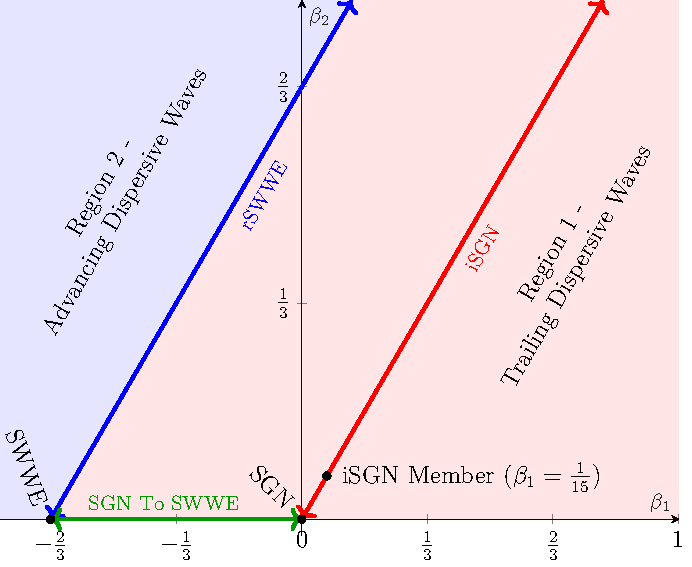
\includegraphics[width=0.4\textwidth]{./Figures/Explanation/BetaPlotAll.pdf}
	\caption{Plot phase speed regions of $\beta_1$ and $\beta_2$ showing important families of equations and particular members of these families.}
	\label{Fig:WaveSpeedReg}
\end{figure}



%-------------------------------------------------
\subsection{Alternative Conservative Form of the gSGN}
%-------------------------------------------------
\citet{Clamond-Dutykh-2018-237} demonstrate how to rearrange \eqref{eq:gSGNuh} for the rSWWE, in an analagous way to the reformulations of SGN demonstrated by []. The purpose of doing this is to remove the mixed spatial-temporal derivative, which is difficult to treat numerically. The reformulation works analogously for the gSGN equations as well, and so we can obtain an equivalent formulation of \eqref{eq:gSGNuh} which becomes
\begin{gather*}\label{eq:G_momentum}
\dfrac{\partial G }{\partial t}  + \dfrac{\partial}{\partial x} \left ( uG + \dfrac{gh^2}{2} - \left(\frac{2}{3} +  \beta_1\right) h^3\dfrac{\partial u}{\partial x}\dfrac{\partial u}{\partial x}  - \frac{1}{2} \beta_2 g h^2  \left[h\frac{\partial^2 h}{\partial x^2} + \frac{1}{2}\frac{\partial h}{\partial x}\frac{\partial h}{\partial x}\right]\right ) = 0.
\end{gather*}
where the new conserved quantity, $G$ is given by
\begin{gather*}
G = hu - \frac{1}{2}\left(\frac{2}{3} + \beta_1\right) \dfrac{\partial }{\partial x} \left ( h^3 \dfrac{\partial u}{\partial x} \right ).
\end{gather*}
Using the appropriate substitution, we can recover the the conserved variable introduced by \citet{Clamond-Dutykh-2018-237} for the rSWWE as well as for the Serre equations []. 

Making this reformulation, we now have the equation of mass for the gSGN and an equation in conservation law form for $G$ which is equivalent to the conservation of momentum equations as follows
\begin{subequations}
\begin{gather}
\dfrac{\partial h}{\partial t} + \dfrac{\partial (uh)}{\partial x} = 0
\label{eq:gSGN_Gh}
\end{gather}
\begin{gather}
\dfrac{\partial G }{\partial t}  + \dfrac{\partial}{\partial x} \left ( uG + \dfrac{gh^2}{2} - \frac{2}{3}\left(1 + \frac{3}{2} \beta_1\right) h^3\dfrac{\partial u}{\partial x}\dfrac{\partial u}{\partial x}  - \frac{1}{2} \beta_2 g h^2  \left[h\frac{\partial^2 h}{\partial x^2} + \frac{1}{2}\frac{\partial h}{\partial x}\frac{\partial h}{\partial x}\right]\right ) = 0.
\label{eq:gSGN_GG}
\end{gather}
with
\begin{gather}\label{eq:G_divergent}
G = uh - \frac{1}{3}\left(1 + \frac{3}{2} \beta_1\right) \dfrac{\partial }{\partial x} \left ( h^3 \dfrac{\partial u}{\partial x} \right ).
\end{gather}
\label{eq:gSGN_G}
\end{subequations}

This form of the equations and a bound on the wave speeds, allows us to solve \eqref{eq:gSGN_G} numerically using a combination of finite difference and finite volume methods as performed in [] for the SGN.


\section{Numerical Method}
The numerical method proposed for the gSGN, is very similar to methods published for the SGN []. For brevity, we will only provide a general overview of the method, whilst highlighting the important differences that need to be made to solve the gSGN over the SGN.

\subsection{Overview}
The numerical method for the gSGN equations proceeds very similarly to the SGN equations, we discretise space into cells of fixed width $\Delta x$, and used fixed time steps $\Delta t$. We then solved 


in particular we have an elliptic equation which relates $h$, $G$ and $u$ and a set of conservation equations for $h$ and $G$. To develop a numerical method for these equations we discretise space into cells of fixed width $\Delta x$, and used fixed time steps $\Delta t$. Using subscripts to denote spatial location, and superscripts to denote time



Following, [] we can therefore solve the gSGN equations using the following method
\begin{enumerate}
	\item We begin with the cell averages $\bar{h}^n_j$ and $\bar{G}^n_j$ for all cells $j$
	\item We solve \eqref{eq:G_divergent} using $\bar{h}^n_j$ and $\bar{G}^n_j$ to obtain an approximation to $u^n_j$ for all cells $j$
	\item We then solve \eqref{eq:gSGN_Gh} and \eqref{eq:gSGN_GG} using a finite volume method with an approximate Riemann solver to obtain $\bar{h}^{n+1}_j$ and $\bar{G}^{n+1}_j$ at the next time step.
\end{enumerate}
Since the finite volume solver is first-order accurate in time, we repeat these steps and do a convex combination to obtain a second-order accurate approximation to \eqref{eq:gSGN_G} in time. 

\subsection{Differences}

\begin{itemize}
	\item Just general form
	\item Highlight changes - limiters on gradients
\end{itemize}

\section{Validation}
\begin{itemize}
	\item Analytic solutions - we recover them (conservation and norm)
	\item Forced solutions - our numerical method can handle any combination of beta values, all terms are approximated with correct order of accuracy. Limiters on gradients off. 
\end{itemize}

\subsection{Analytic Solutions}
\subsubsection{Serre Equations ($\beta_1=\beta_2 =0$) - Solitary Travelling Wave Solution}
When $\beta_1 = \beta_2 = 0$ the gSGN are equivalent to the SGN equations which admit the following travelling wave solution

% xstart  -200.00000000000000     
%xend   200.37505860290673     
%x_len        6400
%n_GhstCells           6
%xbc_len        6412
%dx   6.2509767151117362E-002
%tstart   0.0000000000000000     
%tend   30.000000000000000     
%actual_end_time   30.001639491135400     
%dt   7.6534794620238432E-003
%theta   1.2000000000000000     
%gravity   9.8100000000000005     
%a0   1.0000000000000000     
%a1  0.69999999999999996     
%beta1   0.0000000000000000     
%beta2   0.0000000000000000      


\begin{subequations}
	\begin{equation}
	h(x,t) = a_0 + a_1 \text{sech}^2\left( \kappa (x - ct) \right)
	\end{equation}
	\begin{equation}
	u(x,t) = c \left( 1- \dfrac{a_0}{h(x,t)} \right)
	\end{equation}
	where
	\begin{equation}
	\kappa = \dfrac{\sqrt{3a_1}}{2a_0 \sqrt{a_0 + a_1}}
	\end{equation}
	\begin{equation}
	c = \sqrt{g\left(a_0 + a_1\right)}
	\end{equation}
\end{subequations}


\begin{figure}
	\centering
	\begin{subfigure}{0.32\textwidth}
		\centering
		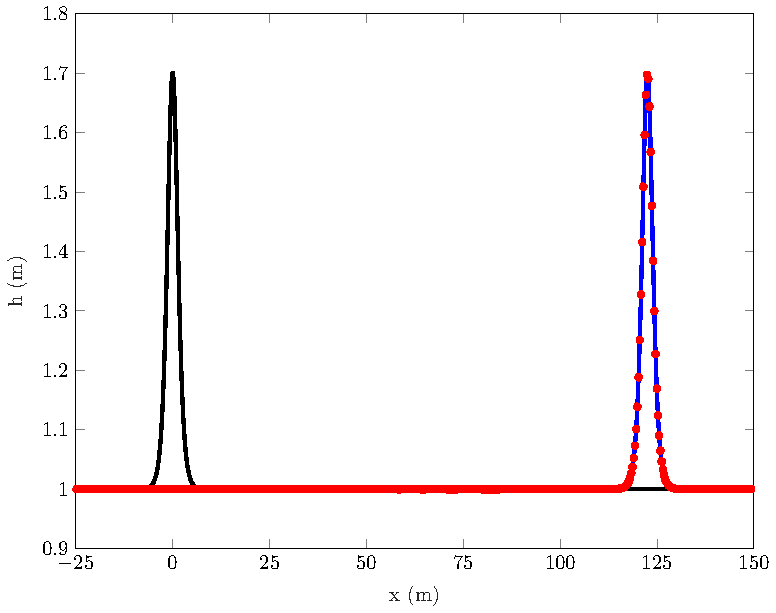
\includegraphics[width=\textwidth]{./Figures/Simulations/Validation/Serre/h.pdf}
		\caption{$h$}
	\end{subfigure}
	\begin{subfigure}{0.32\textwidth}
		\centering
		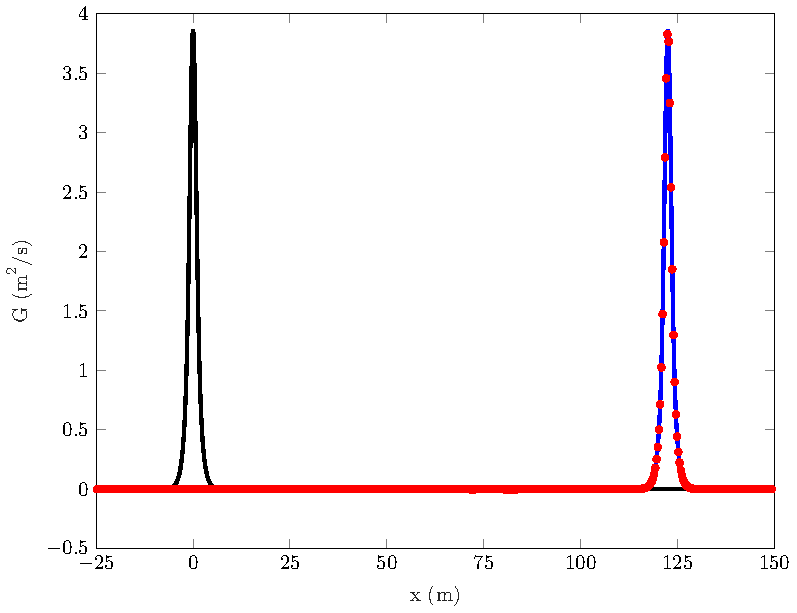
\includegraphics[width=\textwidth]{./Figures/Simulations/Validation/Serre/G.pdf}
		\caption{$G$}
	\end{subfigure}
	\begin{subfigure}{0.32\textwidth}
		\centering
		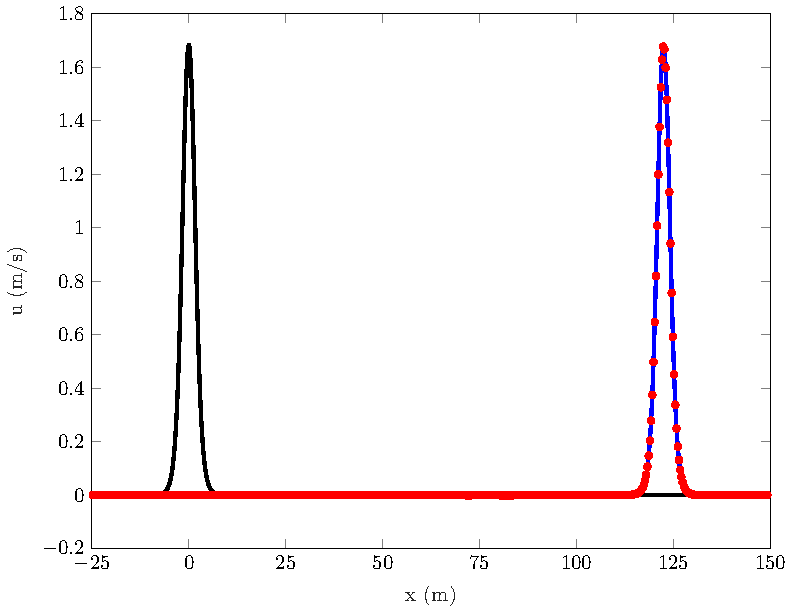
\includegraphics[width=\textwidth]{./Figures/Simulations/Validation/Serre/u.pdf}
		\caption{$u$}
	\end{subfigure}
	\caption{Example plot comparing numerical for $t = 30s$. Initial (\solidrule), analytic solution ({\color{blue}\solidrule}), and numerical solution with $\Delta x \approx 0.06m$ (\tikzcircle{red})  .}
\end{figure}

\begin{figure}
	\centering
	\begin{subfigure}{0.49\textwidth}
		\centering
		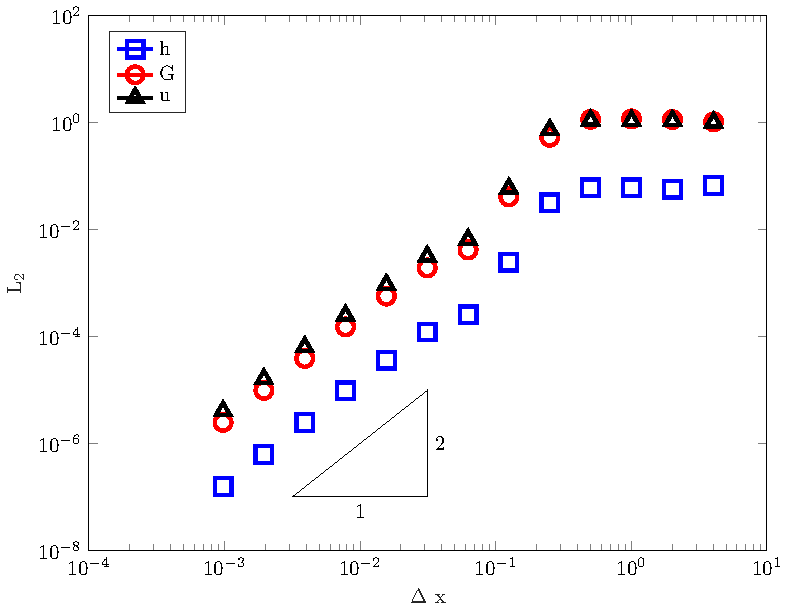
\includegraphics[width=\textwidth]{./Figures/Simulations/Validation/Serre/NormResults.pdf}
		\caption{$L_2$}
	\end{subfigure}
	\begin{subfigure}{0.49\textwidth}
		\centering
		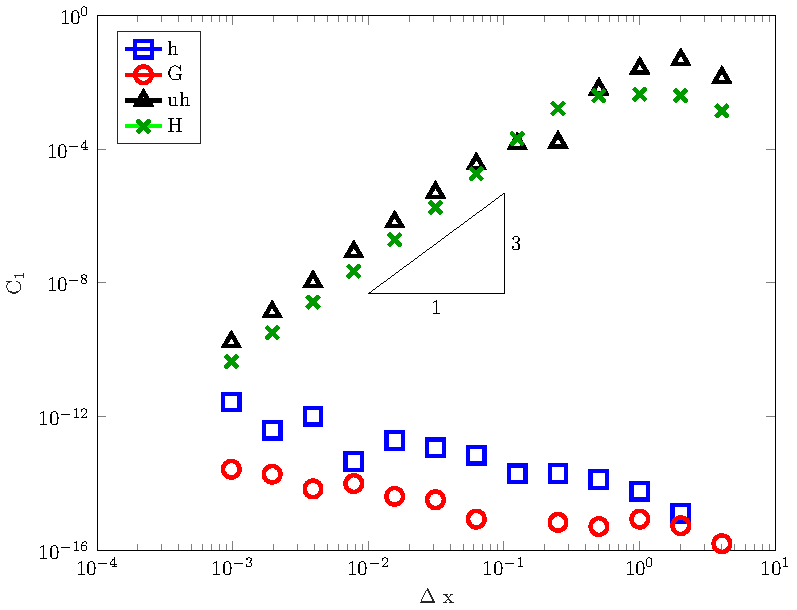
\includegraphics[width=\textwidth]{./Figures/Simulations/Validation/Serre/EnergyResults.pdf}
		\caption{$C_1$, $uh$ (\trianglet{black})}
	\end{subfigure}
	\caption{Convergence and Conservation Plots  $h$ (\squaret{blue}) , $G$ (\circlet{red}), $u$ (\trianglet{black}), $\mathcal{H}$ \crosst{green!60!black}.}
\end{figure}

%% RESULTS %%

Results - Example,Convergence and Conservation Plot

\subsubsection{SWWE ( $\beta_1= -\frac{2}{3}$ and $ \beta_2 =0$ ) - Dambreak Solution }
\begin{align}
h(x,0) & = \left\lbrace \begin{array}{c c}
h_0 & x < 0\\
h_1 & x \ge 0
\end{array} \right.  \\
u(x,0) &= 0 \\
G(x,0) &= 0
\end{align}

%xstart  -250.00000000000000     
%xend   250.18751171948242     
%x_len       16000
%n_GhstCells           6
%xbc_len       16012
%dx   3.1251953247077940E-002
%tstart   0.0000000000000000     
%tend   35.000000000000000     
%actual end time   35.002559302559774     
%dt   2.8803949393156393E-003
%theta   1.2000000000000000     
%gravity   9.8100000000000005     
%hl   2.0000000000000000     
%hr   1.0000000000000000     
%beta1 -0.66666666666666663     
%beta2   0.0000000000000000     

We have an analytic solution for the SWWE for the discontinuous limit of these equations as $\alpha \rightarrow 0$. It is 3 constant states $(h_0,0)$, $(h_s,u_s)$ and $(h_1,0)$ where
\begin{equation}
h_s = \dfrac{h_0}{2} \left[  \sqrt{1 + 8 \left( \dfrac{2 h_s}{h_s - h_0} \left(\dfrac{\sqrt{gh_1} - \sqrt{gh_s}}{\sqrt{gh_0}}\right)\right)^2 } - 1 \right]
\end{equation}
\begin{equation}
u_s = 2\left(\sqrt{gh_1} - \sqrt{gh_s} \right).
\end{equation}
Where $(h_0,0)$ and $(h_s,u_s)$ are joined by a 

\begin{figure}
	\centering
	\begin{subfigure}{0.32\textwidth}
		\centering
		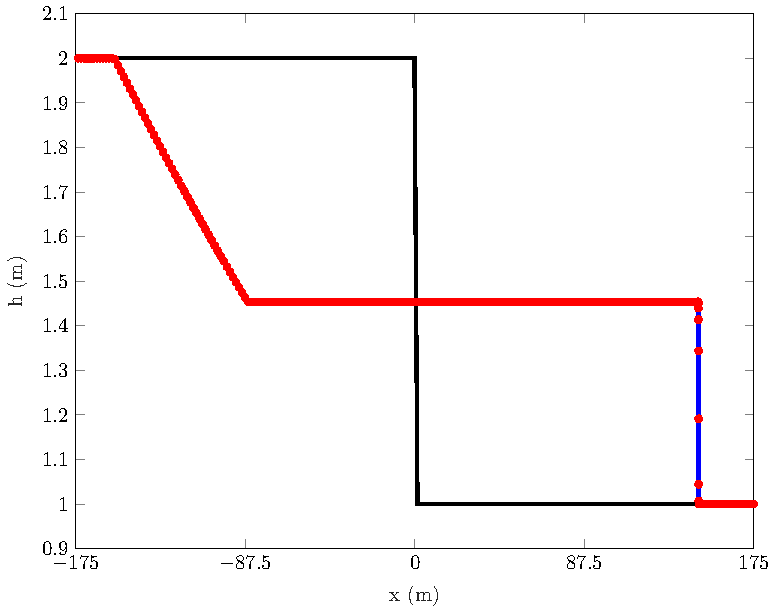
\includegraphics[width=\textwidth]{./Figures/Simulations/Validation/DBSWWE/h.pdf}
		\caption{$h$}
	\end{subfigure}
	\begin{subfigure}{0.32\textwidth}
		\centering
		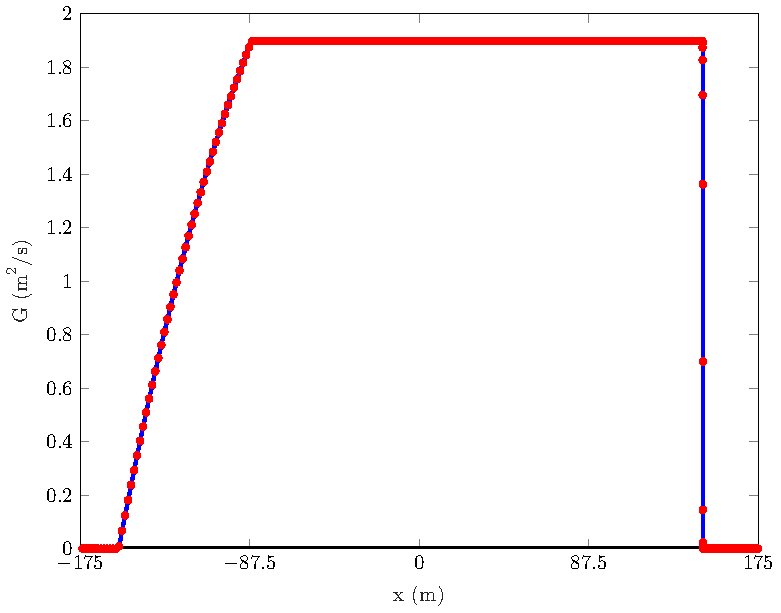
\includegraphics[width=\textwidth]{./Figures/Simulations/Validation/DBSWWE/G.pdf}
		\caption{$G$}
	\end{subfigure}
	\begin{subfigure}{0.32\textwidth}
		\centering
		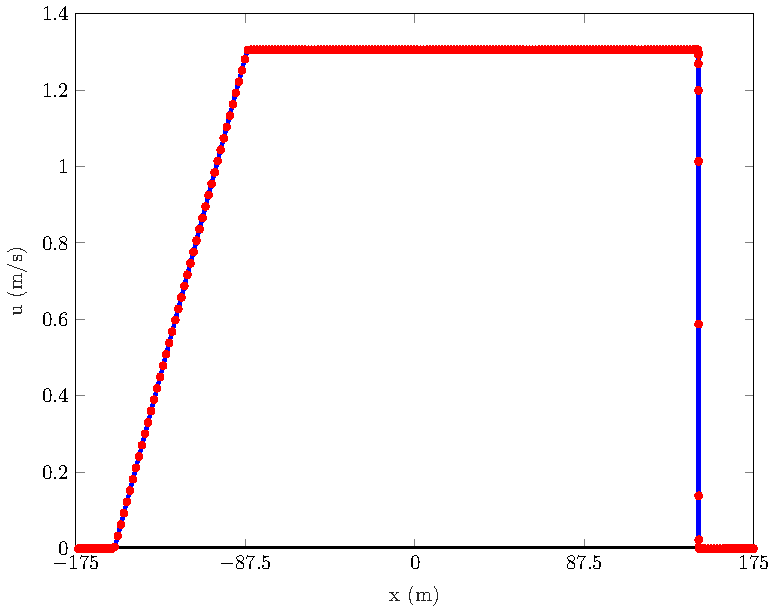
\includegraphics[width=\textwidth]{./Figures/Simulations/Validation/DBSWWE/u.pdf}
		\caption{$u$}
	\end{subfigure}
	\caption{Example plots for $t=35s$. Initial (\solidrule), analytic solution ({\color{blue}\solidrule}), and numerical solution with $\Delta x \approx 0.03m$ (\tikzcircle{red})  .}
\end{figure}



\begin{figure}
	\centering
	\begin{subfigure}{0.45\textwidth}
		\centering
		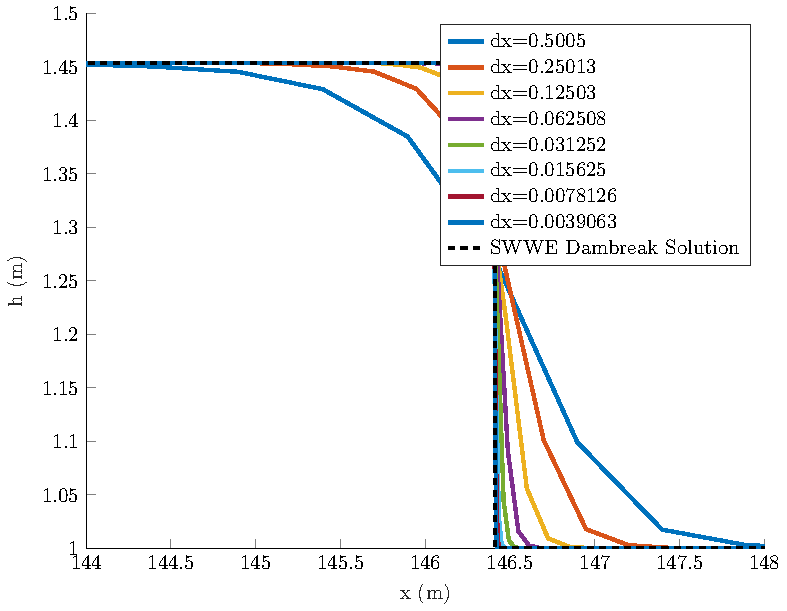
\includegraphics[width=\textwidth]{./Figures/Simulations/Validation/DBSWWE/hFront.pdf}
		\caption{$h$}
	\end{subfigure}
	\begin{subfigure}{0.45\textwidth}
		\centering
		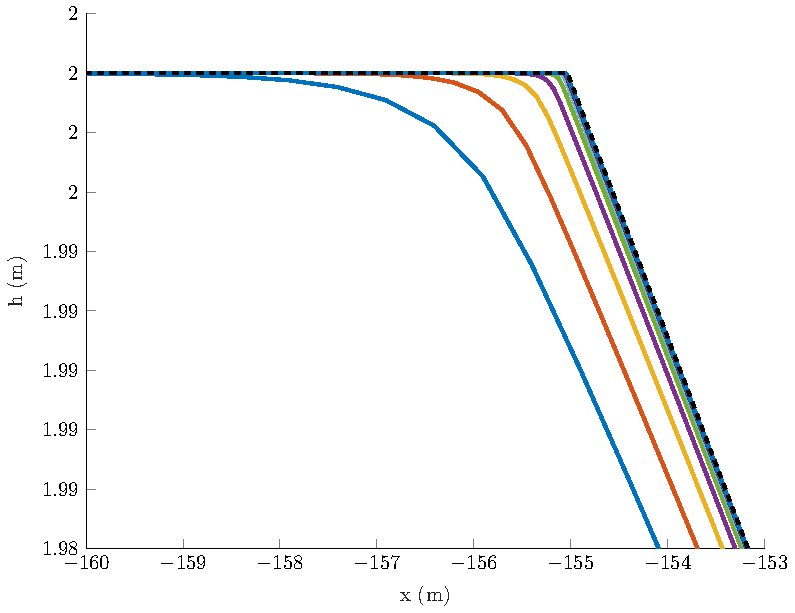
\includegraphics[width=\textwidth]{./Figures/Simulations/Validation/DBSWWE/hRFTop.pdf}
		\caption{$h$}
	\end{subfigure}
	\caption{Example plots for $t=35s$. Initial (\solidrule), analytic solution ({\color{blue}\solidrule}), and numerical solution with $\Delta x \approx 0.03m$ (\tikzcircle{red})  .}
\end{figure}

\begin{figure}
	\centering
	\begin{subfigure}{0.49\textwidth}
		\centering
		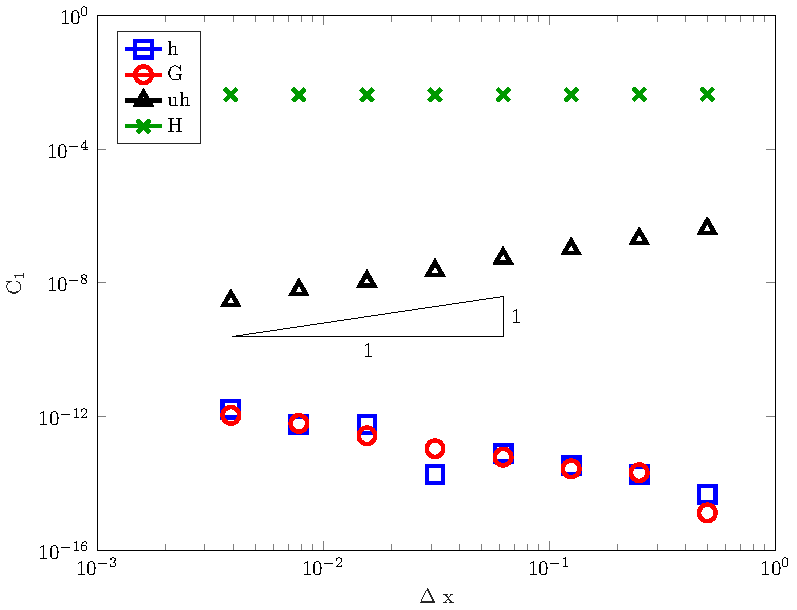
\includegraphics[width=\textwidth]{./Figures/Simulations/Validation/DBSWWE/EnergyResults.pdf}
		\caption{}
	\end{subfigure}
	\caption{Conservation Plots  $h$ (\squaret{blue}) , $G$ (\circlet{red}), $uh$ (\trianglet{black}), $\mathcal{H}$ \crosst{green!60!black}.}
\end{figure}

\begin{figure}
	\centering
	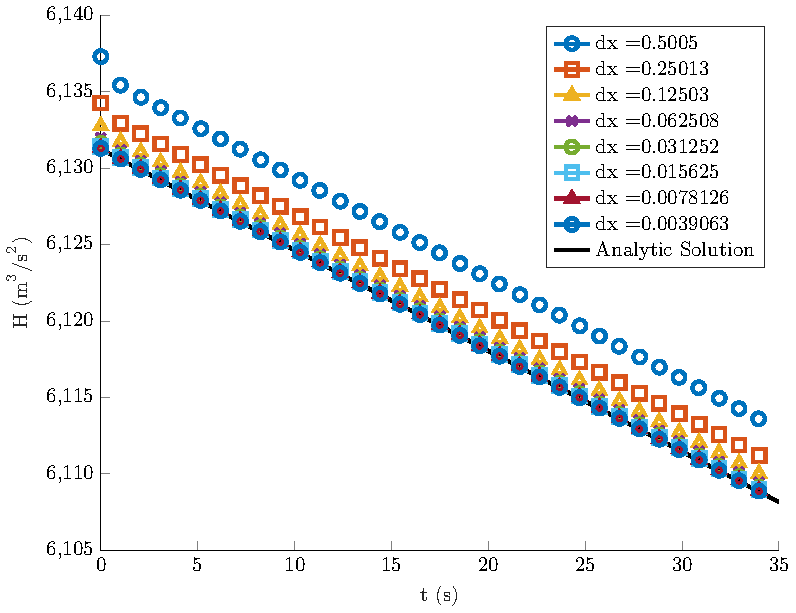
\includegraphics[width=0.49\textwidth]{./Figures/Simulations/Validation/DBSWWE/EnergyOverTime.pdf}
	\caption{Plot of $\mathcal{H}$ over time.}
\end{figure}


Results - Example and Conservation Table


\subsection{Forced Solutions}
To demonstrate the validity and versatility of our method to solve the gSGN whilst allowing varying $\beta_i$ values, we make use of forced solutions. To generate a forced solution we consider the modified gSGN equations 

\begin{subequations}
	\begin{gather}
	\dfrac{\partial h}{\partial t} + \dfrac{\partial (uh)}{\partial x} = \dfrac{\partial h^*}{\partial t} + \dfrac{\partial (u^*h^*)}{\partial x} 
	\label{eq:gSGN_Gh_Forced}
	\end{gather}
	\begin{multline}
	\dfrac{\partial G }{\partial t}  + \dfrac{\partial}{\partial x} \left ( uG + \dfrac{gh^2}{2} - \frac{2}{3}\left(1 + \frac{3}{2} \beta_1\right) h^3\dfrac{\partial u}{\partial x}\dfrac{\partial u}{\partial x}  - \frac{1}{2} \beta_2 g h^2  \left[h\frac{\partial^2 h}{\partial x^2} + \frac{1}{2}\frac{\partial h}{\partial x}\frac{\partial h}{\partial x}\right]\right ) = \\ \dfrac{\partial G^* }{\partial t}  + \dfrac{\partial}{\partial x} \left ( u^*G^* + \dfrac{g\left(h^*\right)^2}{2} - \frac{2}{3}\left(1 + \frac{3}{2} \beta_1\right) \left(h^*\right)^3\dfrac{\partial u^*}{\partial x}\dfrac{\partial u^*}{\partial x}  - \frac{1}{2} \beta_2 g \left(h^*\right)^2  \left[h^*\frac{\partial^2 h^*}{\partial x^2} + \frac{1}{2}\frac{\partial h^*}{\partial x}\frac{\partial h^*}{\partial x}\right]\right ) 
	\label{eq:gSGN_GG_Forced}
	\end{multline}
\end{subequations}

which admit the solutions $h^*$, $u^*$ and $G^*$ assuming $G^*$ appropriately satisfies \eqref{eq:G_divergent}. Since these equations are satisfied for any chosen $h^*$, $u^*$ and $G^*$, we can generated any desired solution. Since the left hand-side of these modified equations are approximated by our numerical method, if we combine the numerical method with analytic expressions for the right handside, we have a method that approximates the forced gSGN equation with the same convergence properties as the underlying numerical method for the gSGN equations. 

Since we are free to choose $h^*$, $u^*$ and $G^*$ we can generate solutions and thus test our convergence properties for situations for which no analytic solution to the equations exist, in particular in this paper we are interested in solutions where the $\beta$ values vary in space and time. 

I have used this technique to investigate the method for the following forced solutions

\begin{subequations}
	\begin{equation}
	h^*(x,t) = a_0 + a_1 \exp\left( \dfrac{\left(x - a_2 t\right)^2}{2 a_3} \right)
	\end{equation}
	\begin{equation}
	u^*(x,t) = a_4 \exp\left( \dfrac{\left(x - a_2 t\right)^2}{2 a_3} \right)
	\end{equation}
	\begin{align}
	\beta_1(x,t) &= a_6 \\
	\beta_2(x,t) &= a_7
	\end{align}
\end{subequations}
where $G^*$ is determined by \eqref{eq:G_divergent} with the above values. 


% xstart :  -100.00000000000000     
%xend :   100.00000000000000     
%xbc_len :        6412
%dx = (x_end - x_start) / (x_len -1)  :   3.1254883575558681E-002
%n_GhstCells :           6
%tstart :   0.0000000000000000     
%tend :   10.000000000000000     
%actual end time :   10.000952459292289     
%dt/dx :   5.2619712865493169E-002
%dt = dx*(dt/dx)  :   1.6446229993903163E-003
%gravity :   9.8100000000000005     
%theta :   1.2000000000000000     
%a0 :   1.0000000000000000     
%a1 :  0.50000000000000000     
%a2 :   5.0000000000000000     
%a3 :   20.000000000000000     
%a4 :  0.29999999999999999     
%a5 :   0.0000000000000000     
%b1a6 :   0.0000000000000000     
%b1a7 :   1.0000000000000000     
%b2a6 :   0.0000000000000000     
%b2a7 :   2.0000000000000000     

\begin{figure}
	\centering
	\begin{subfigure}{0.32\textwidth}
		\centering
		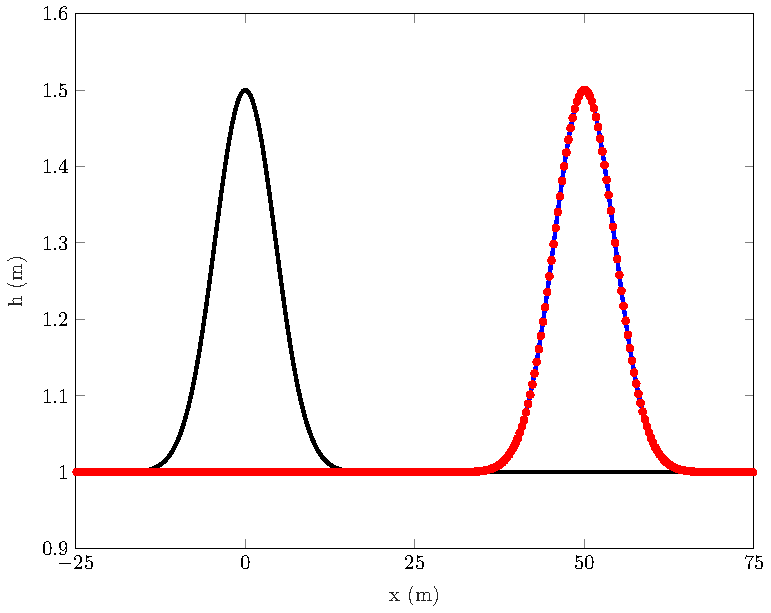
\includegraphics[width=\textwidth]{./Figures/Simulations/Validation/Forced/h.pdf}
		\caption{$h$}
	\end{subfigure}
	\begin{subfigure}{0.32\textwidth}
		\centering
		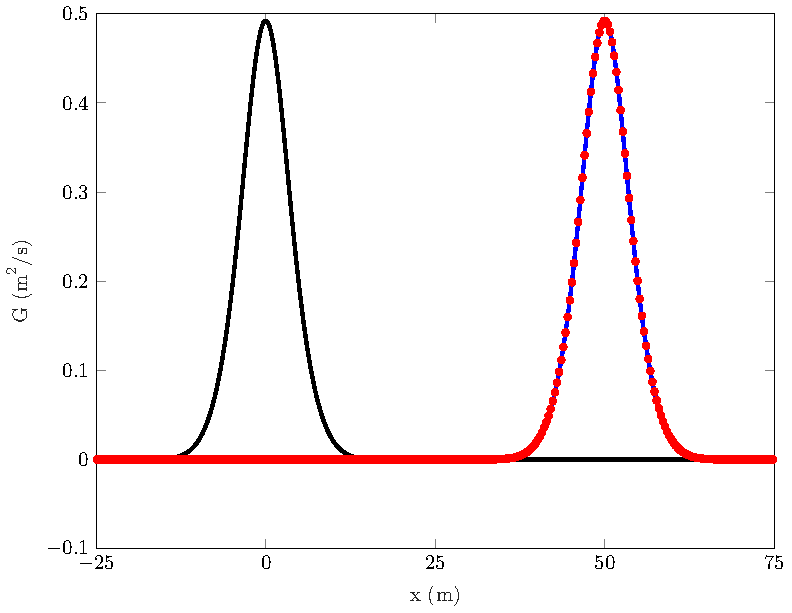
\includegraphics[width=\textwidth]{./Figures/Simulations/Validation/Forced/G.pdf}
		\caption{$G$}
	\end{subfigure}
	\begin{subfigure}{0.32\textwidth}
		\centering
		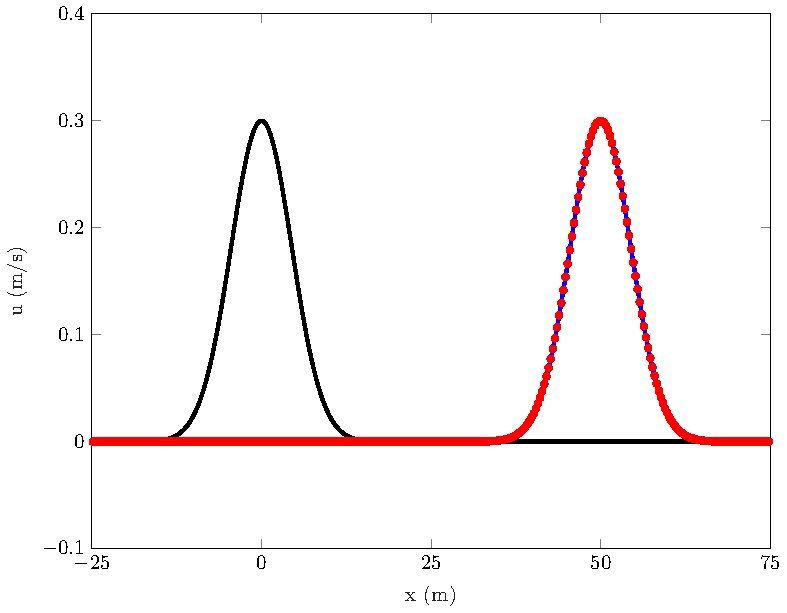
\includegraphics[width=\textwidth]{./Figures/Simulations/Validation/Forced/u.pdf}
		\caption{$u$}
	\end{subfigure}
	\caption{Example plots Initial (\solidrule), analytic solution ({\color{blue}\solidrule}), and numerical solution with $\Delta x \approx 0.03m$ (\tikzcircle{red})  .}
\end{figure}

\begin{figure}
	\centering
	\begin{subfigure}{0.49\textwidth}
		\centering
		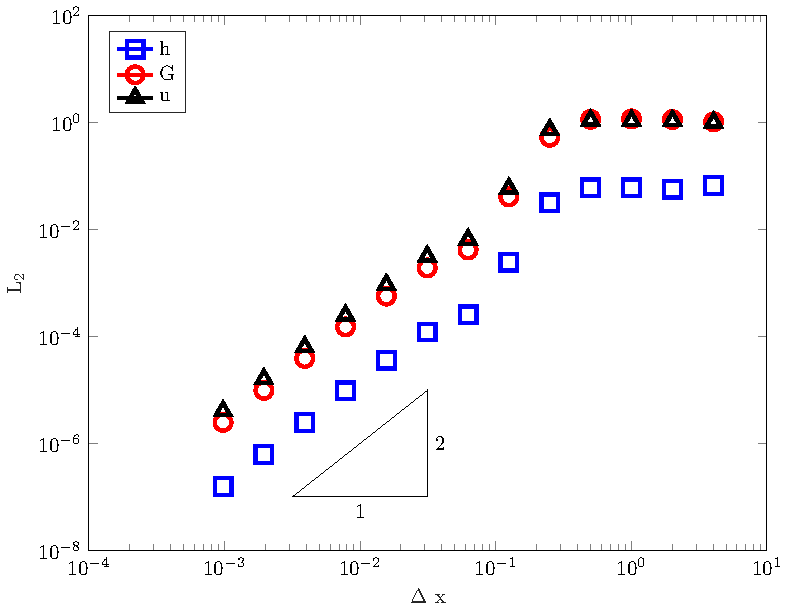
\includegraphics[width=\textwidth]{./Figures/Simulations/Validation/Serre/NormResults.pdf}
		\caption{$L_2$}
	\end{subfigure}
	\caption{Convergence and Conservation Plots  $h$ (\squaret{blue}) , $G$ (\circlet{red}), $u$ (\trianglet{black}).}
\end{figure}

Results - Example plot and L1 convergence, comment that this worked for all beta values, and we only show one for conciseness


\section{Smooth Dambreak Study}
\begin{align}
h(x,0) & = h_0 + \dfrac{h_1 - h_0}{2} \left(1 + \tanh\left(\dfrac{x}{\alpha}\right)\right)  \\
u(x,0) &= 0 \\
G(x,0) &= 0
\end{align}


\subsection{Regularised SWWE Family $\beta_2 = \frac{2}{3} + \beta_1$}
Justify interest, cite denys paper on regularised SWWE

% xstart :  -250.00000000000000     
%xend :   250.04687573243325     
%x_len :       64000
%n_GhstCells :           6
%xbc_len :       64012
%dx = (x_end - x_start) / (x_len -1)  :   7.8126220722198776E-003
%tstart :   0.0000000000000000     
%tend :   35.000000000000000     
%actual end time :   35.000198467001518     
%dt:   7.2006497967329038E-004
%gravity :   9.8100000000000005     
%hl :   2.0000000000000000     
%hr :   1.0000000000000000     
%dbalpha :  0.10000000000000001     
%beta1 : -0.66666666666666663     
%beta2 :   0.0000000000000000   

\begin{itemize}
	\item we do get nice well behaved transitions between behaviours when varying $\beta$ values
	we get nice convergence.
	\item Although solutions look nice in h, in G there can be quite large values in the smoothed regions. However, u still looks quite nice. 
\end{itemize}

\begin{figure}
	\centering
	\begin{subfigure}{0.32\textwidth}
		\centering
		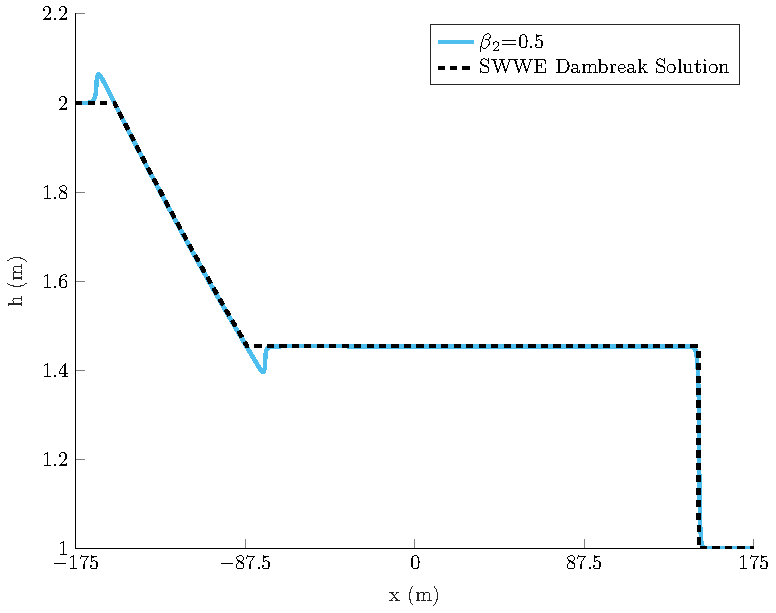
\includegraphics[width=\textwidth]{./Figures/Simulations/Study/RegSWWE/Convergence/h.pdf}
		\caption{$h$}
	\end{subfigure}
	\begin{subfigure}{0.32\textwidth}
	\centering
	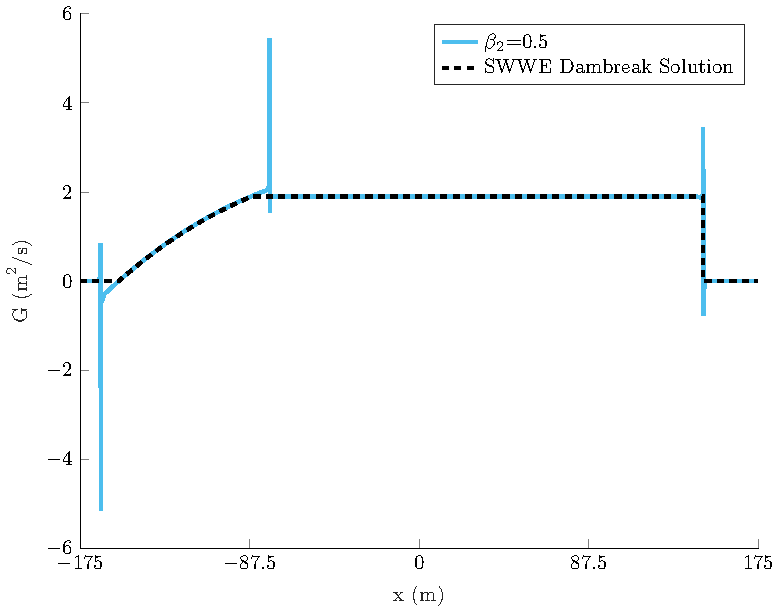
\includegraphics[width=\textwidth]{./Figures/Simulations/Study/RegSWWE/Convergence/G.pdf}
	\caption{$G$}
	\end{subfigure}
	\begin{subfigure}{0.32\textwidth}
	\centering
	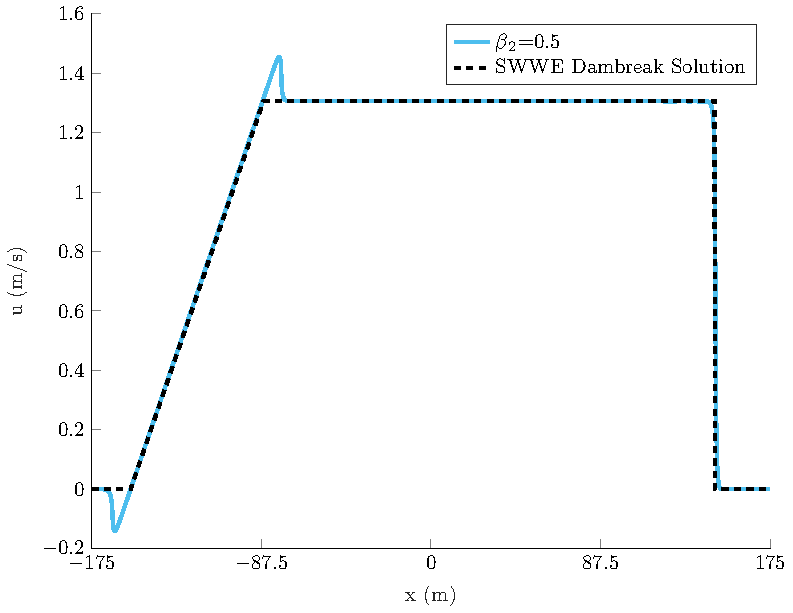
\includegraphics[width=\textwidth]{./Figures/Simulations/Study/RegSWWE/Convergence/u.pdf}
	\caption{$u$}
	\end{subfigure}
	\caption{Plot of example numerical solution for representative memeber of regularised SWWE family to smooth dambreak problem at $t=35s$.}
\end{figure}

\begin{figure}
	\centering
	\begin{subfigure}{0.32\textwidth}
		\centering
		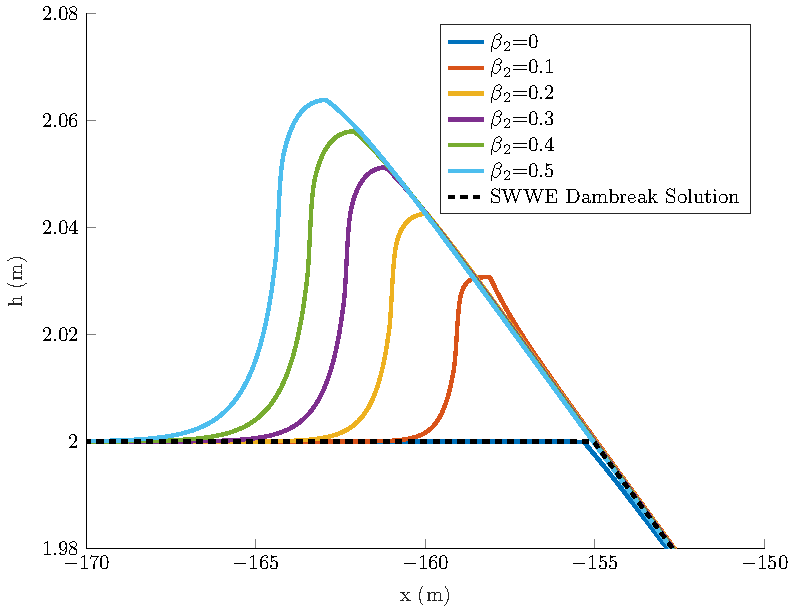
\includegraphics[width=\textwidth]{./Figures/Simulations/Study/RegSWWE/Convergence/hRFtop.pdf}
		\caption{$h$ top of rarefaction fan}
	\end{subfigure}
	\begin{subfigure}{0.32\textwidth}
		\centering
		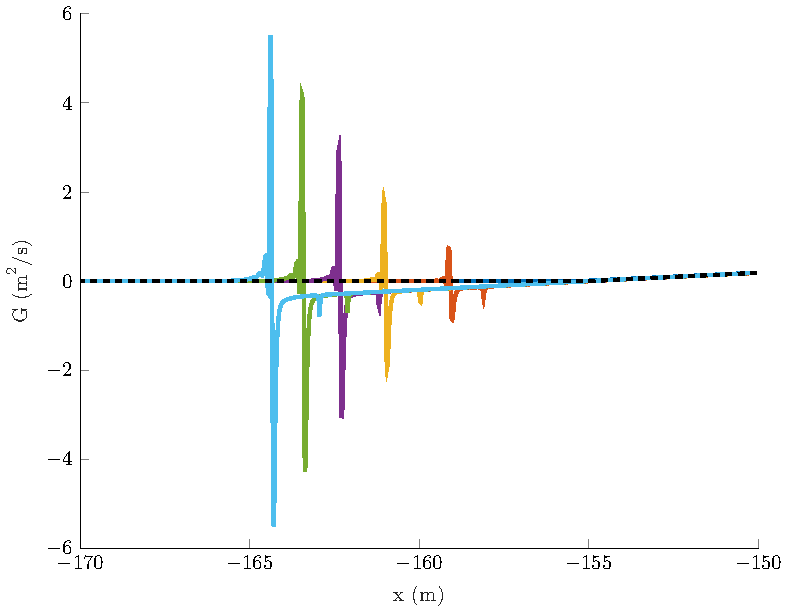
\includegraphics[width=\textwidth]{./Figures/Simulations/Study/RegSWWE/Convergence/GRFtop.pdf}
		\caption{$G$ top of rarefaction fan}
	\end{subfigure}
	\begin{subfigure}{0.32\textwidth}
		\centering
		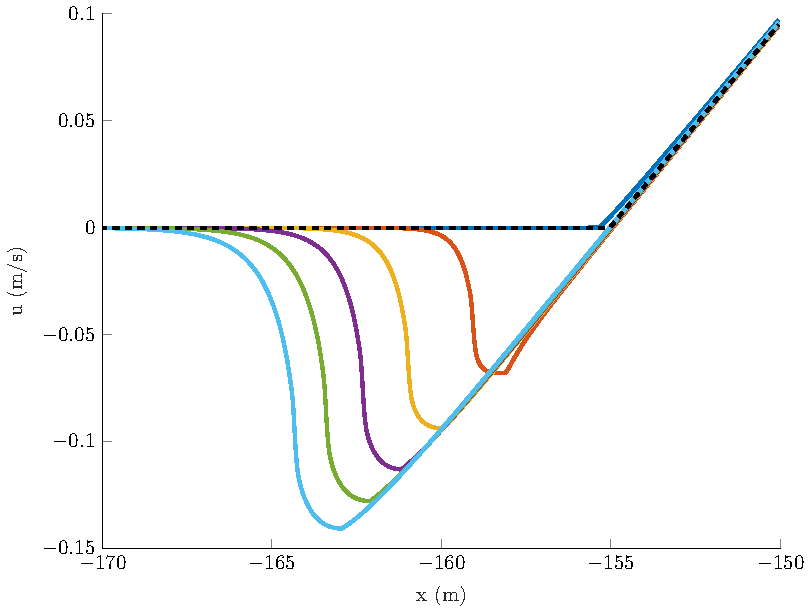
\includegraphics[width=\textwidth]{./Figures/Simulations/Study/RegSWWE/Convergence/uRFtop.pdf}
		\caption{$u$ top of rarefaction fan}
	\end{subfigure}
	\begin{subfigure}{0.32\textwidth}
	\centering
	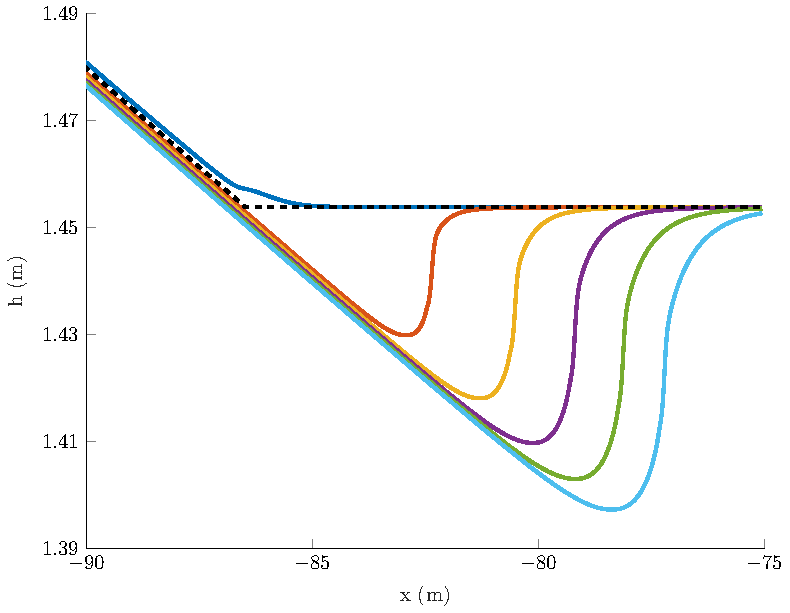
\includegraphics[width=\textwidth]{./Figures/Simulations/Study/RegSWWE/Convergence/hRFBot.pdf}
	\caption{$h$ bottom of rarefaction fan}
	\end{subfigure}
	\begin{subfigure}{0.32\textwidth}
	\centering
	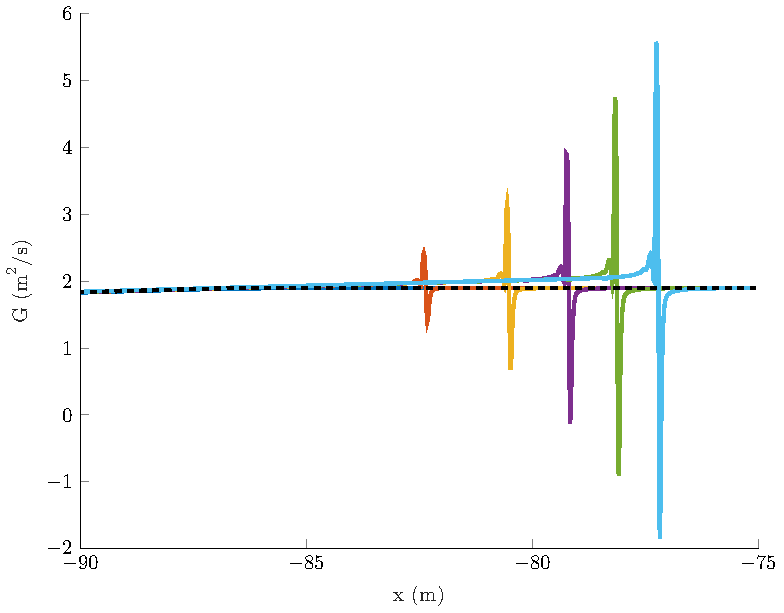
\includegraphics[width=\textwidth]{./Figures/Simulations/Study/RegSWWE/Convergence/GRFBot.pdf}
	\caption{$G$ bottom of rarefaction fan}
	\end{subfigure}
	\begin{subfigure}{0.32\textwidth}
	\centering
	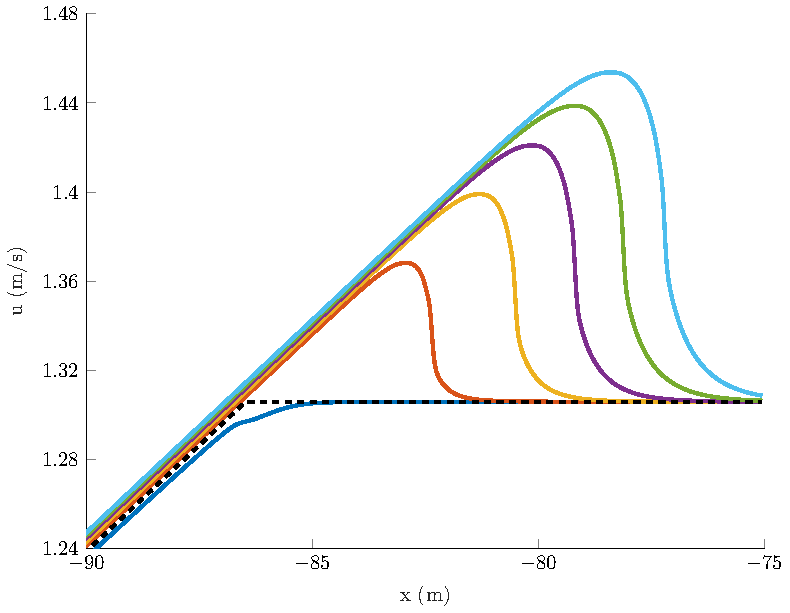
\includegraphics[width=\textwidth]{./Figures/Simulations/Study/RegSWWE/Convergence/uRFBot.pdf}
	\caption{$u$ bottom  of rarefaction fan}
	\end{subfigure}
	\begin{subfigure}{0.32\textwidth}
	\centering
	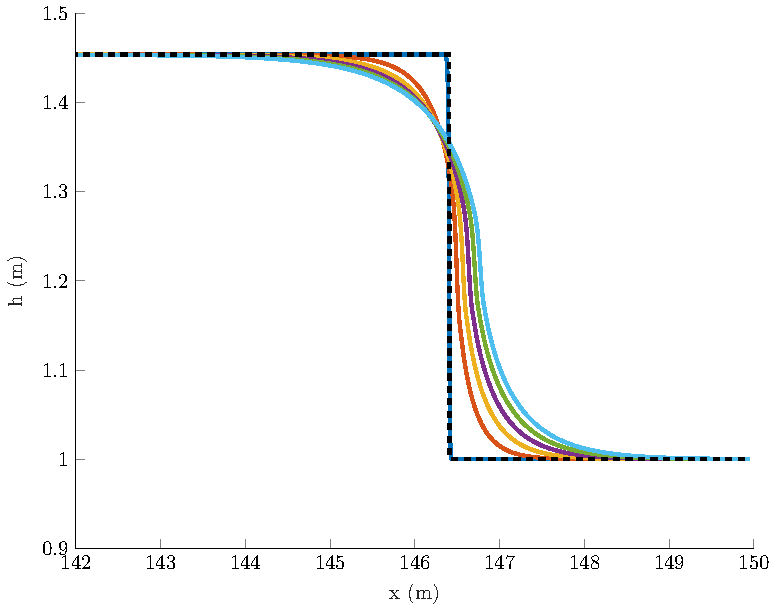
\includegraphics[width=\textwidth]{./Figures/Simulations/Study/RegSWWE/Convergence/hFront.pdf}
	\caption{$h$ shock front}
	\end{subfigure}
	\begin{subfigure}{0.32\textwidth}
	\centering
	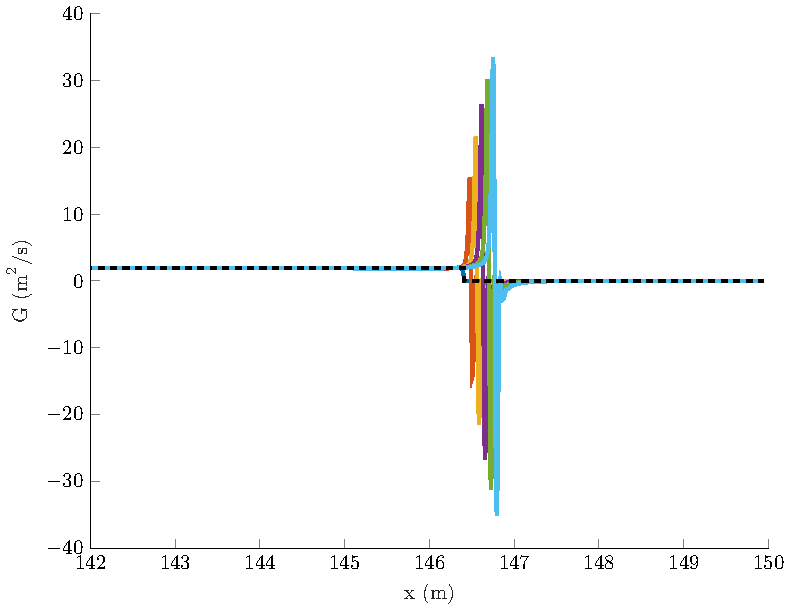
\includegraphics[width=\textwidth]{./Figures/Simulations/Study/RegSWWE/Convergence/GFront.pdf}
	\caption{$G$ shock front}
	\end{subfigure}
	\begin{subfigure}{0.32\textwidth}
	\centering
	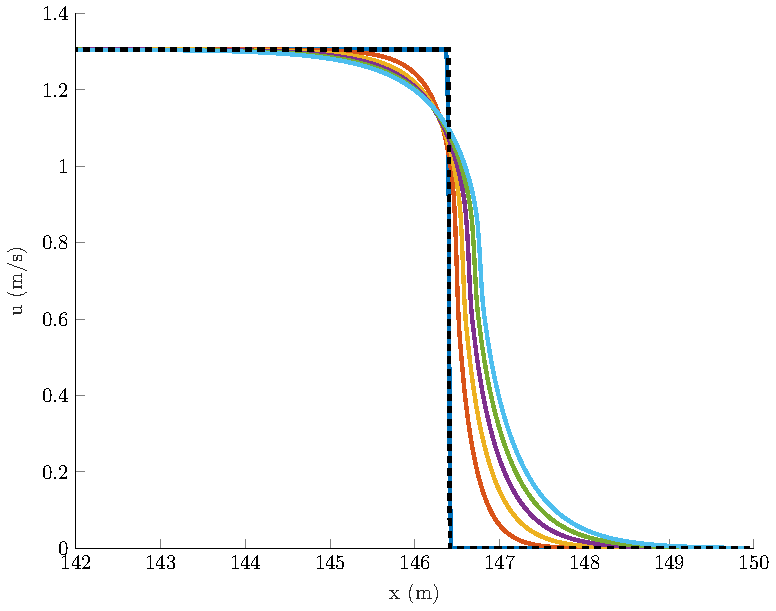
\includegraphics[width=\textwidth]{./Figures/Simulations/Study/RegSWWE/Convergence/uFront.pdf}
	\caption{$u$ shock front}
	\end{subfigure}

	\caption{Plot of multiple smooth dambreak numerical solutions at $t=35s$. $\beta_2 = 0$ ({\color{mycolor1} \solidrule}), $\beta_2 = 0.1$ ({\color{mycolor2} \solidrule}), $\beta_2 = 0.2$ ({\color{mycolor3} \solidrule}), $\beta_2 = 0.3$ ({\color{mycolor4} \solidrule}), $\beta_2 = 0.4$ ({\color{mycolor5} \solidrule}), $\beta_2 = 0.5$ ({\color{mycolor6} \solidrule}).} 
\end{figure}



\begin{table}
	\centering
	\begin{tabular}{c | c}
		Colour region & Condition \\
		\hline
		first blue & $\dfrac{x}{t} \le u_{s} - \sqrt{g h_{s}} $ \\
		first red & $  u_{s} - \sqrt{g h_{s}} \le \dfrac{x}{t} \le u_s - \sqrt{gh_s} \sqrt{\dfrac{\beta_2}{\frac{2}{3} + \beta_1}}$ \\
		first green & $u_s - \sqrt{gh_s} \sqrt{\dfrac{\beta_2}{\frac{2}{3} + \beta_1}} \le \dfrac{x}{t} \le u_{s}$ \\
		second green & $u_{s} \le \dfrac{x}{t}\le u_s + \sqrt{gh_s} \sqrt{\dfrac{\beta_2}{\frac{2}{3} + \beta_1}}$ \\
		second red & $  u_s + \sqrt{gh_s} \sqrt{\dfrac{\beta_2}{\frac{2}{3} + \beta_1}} \le \dfrac{x}{t} \le  u_{s} + \sqrt{g h_{s}} $ \\
		second blue & $u_{s} +  \sqrt{g h_{s}} \le \dfrac{x}{t} $ 	
	\end{tabular}
	\caption{Regions for plots.  	\label{tab:regions1}  }
\end{table}

\begin{figure}
	\centering
	\begin{subfigure}{0.49\textwidth}
		\centering
		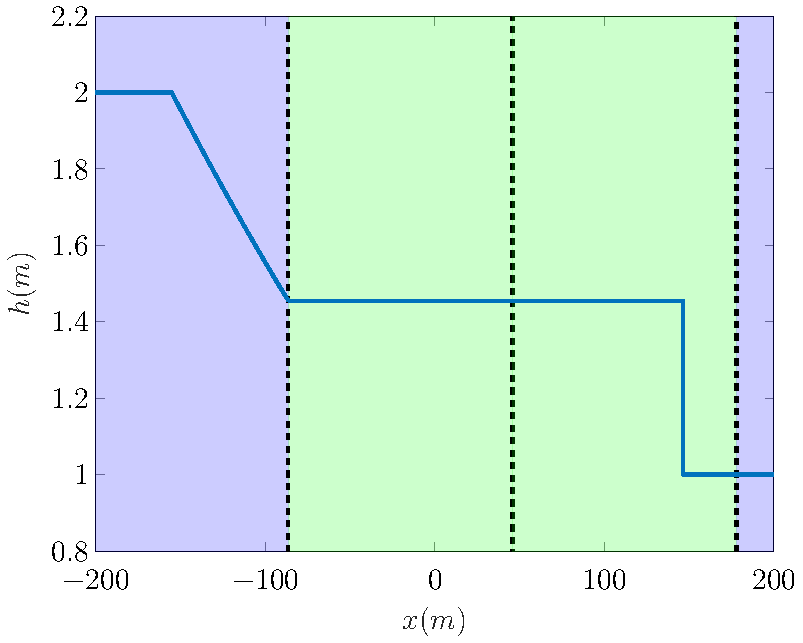
\includegraphics[width=\textwidth]{./Figures/Simulations/Study/RegSWWE/Regions/hRegionsSWWE.pdf}
		\caption{$\beta_2 = 0$}
	\end{subfigure}
	\begin{subfigure}{0.49\textwidth}
		\centering
		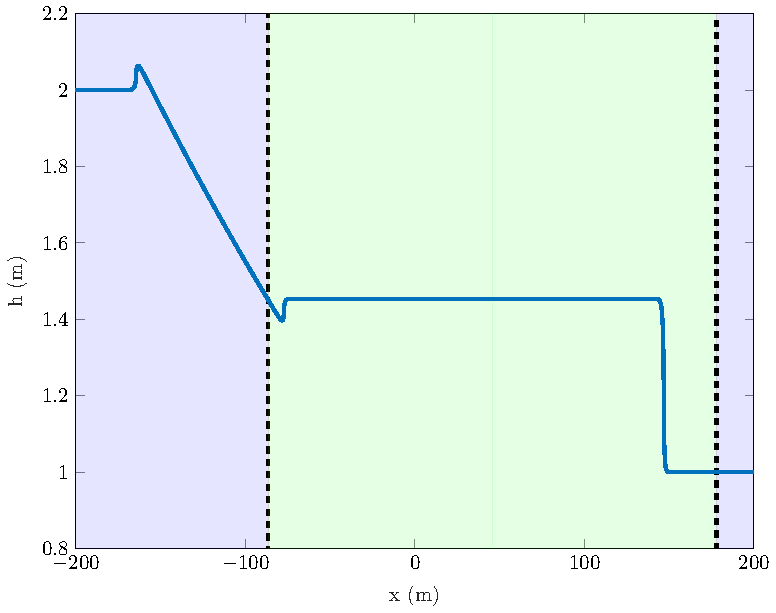
\includegraphics[width=\textwidth]{./Figures/Simulations/Study/RegSWWE/Regions/hRegionsREGSWWE.pdf}
		\caption{$\beta_2 = 0.5$}
	\end{subfigure}
	\caption{Regions of wave speeds for the smooth dambreak numerical solution at $t=35s$.}
\end{figure}

\begin{table}
	\centering
	\begin{tabular}{ c | c | c | c | c }
	$\beta_2$ & $h$ & $G$ & $uh$ & $\mathcal{H}$  \\
		\hline
	\T $0$ &	$5.8 \times 10^{-13}$ & $6.3 \times 10^{-13}$  & $6.3 \times 10^{-9}$ &	 $3.7 \times 10^{-3}$ \\
	\T $0.1$ &	$6.4 \times 10^{-13}$ & $6.4 \times 10^{-13}$  & $9.8 \times 10^{-6}$ &	 $3.9 \times 10^{-3}$ \\
	\T $0.2$ &	$6.7 \times 10^{-13}$ & $6.4 \times 10^{-13}$  & $1.1\times 10^{-5}$ &	 $4.1 \times 10^{-3}$ \\
	\T $0.3$ &	$6.9 \times 10^{-13}$ & $6.4 \times 10^{-13}$  & $1.2\times 10^{-5}$ &	 $4.3 \times 10^{-3}$ \\
	\T $0.4$ &	$7.1 \times 10^{-13}$ & $6.6 \times 10^{-13}$  & $1.2\times 10^{-5}$ &	 $4.4 \times 10^{-3}$ \\
	\T $0.5$ &	$7.1 \times 10^{-13}$ & $6.5 \times 10^{-13}$  & $1.3\times 10^{-5}$ &	 $4.6 \times 10^{-3}$ \\
	\end{tabular}
	\caption{Conservation errors for Regularised SWWE for the solutions provided above with $\beta_1 = \beta_2 - \frac{2}{3}$.}
\end{table}


\begin{figure}
	\centering
	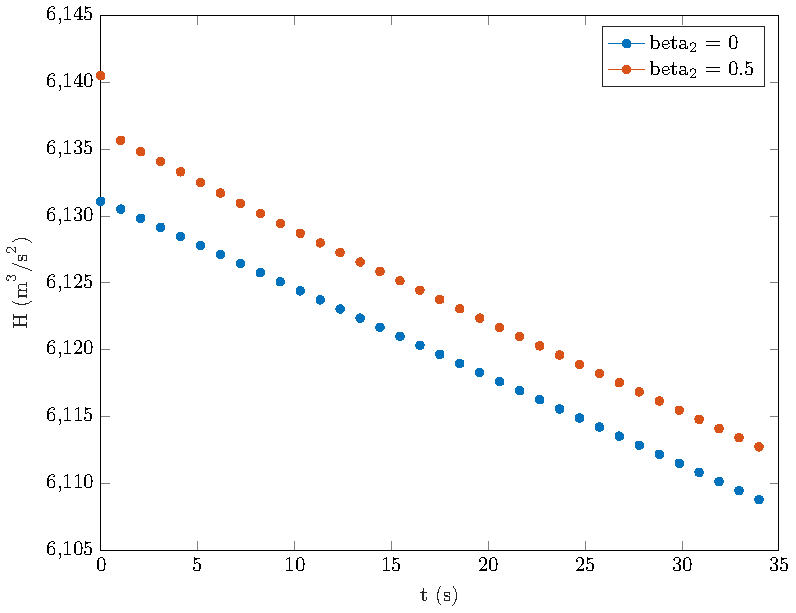
\includegraphics[width=0.6\textwidth]{./Figures/Simulations/Study/RegSWWE/Energy/EnergyOverTime.pdf}
	\caption{Energy over time for the numerical solutions, for the $\beta$ values in the Regularised SWWE family.}
\end{figure}


\subsection{Modified Dispersion Serre Family $\beta_2 = \beta_1$}
Justify interest, cite denys paper on dispersion modified equations

Points:
\begin{itemize}
	\item we do get nice well behaved transitions between behaviours when varying $\beta$
	\item Dispersive wave train location well approximated by using the linear wave speeds. Although the bump around these bounds suggests non-linear effects are important as well, particularly close to transitions across the wavespeed boundaries. 
	\item Improved dispersion may better approximate the dispsersion relation when $k\ll 1$, but at the cost of the middle of the dispersive wave train
	\item We get the bump behaviour observed in the db paper, but now dispersive wave trains are separate.
	\item Conservation is pretty similar, except for energy where it gets worse - this suggests that we will need finer grids to get good solutions particularly when gradients are large.
\end{itemize}

\begin{figure}
	\centering
	\begin{subfigure}{0.322\textwidth}
		\centering
		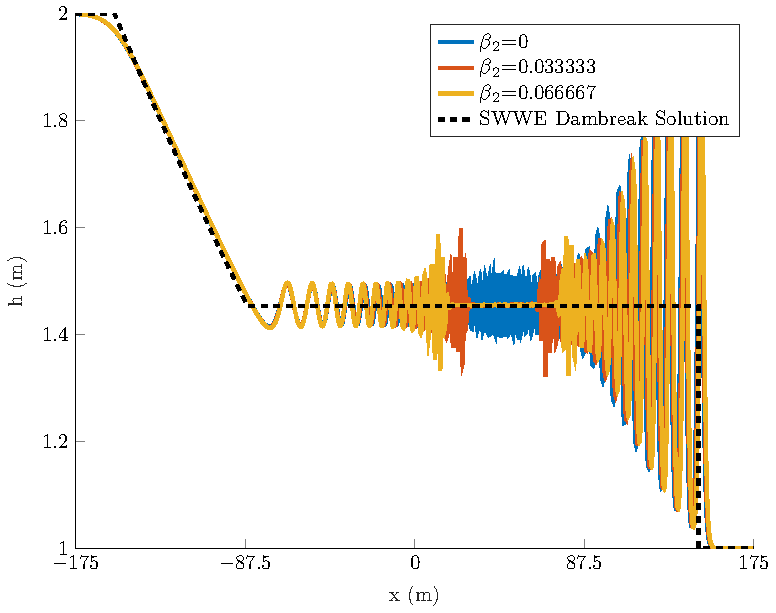
\includegraphics[width=\textwidth]{./Figures/Simulations/Study/ImpDisp/h.pdf}
		\caption{$h$}
	\end{subfigure}
	\begin{subfigure}{0.32\textwidth}
		\centering
		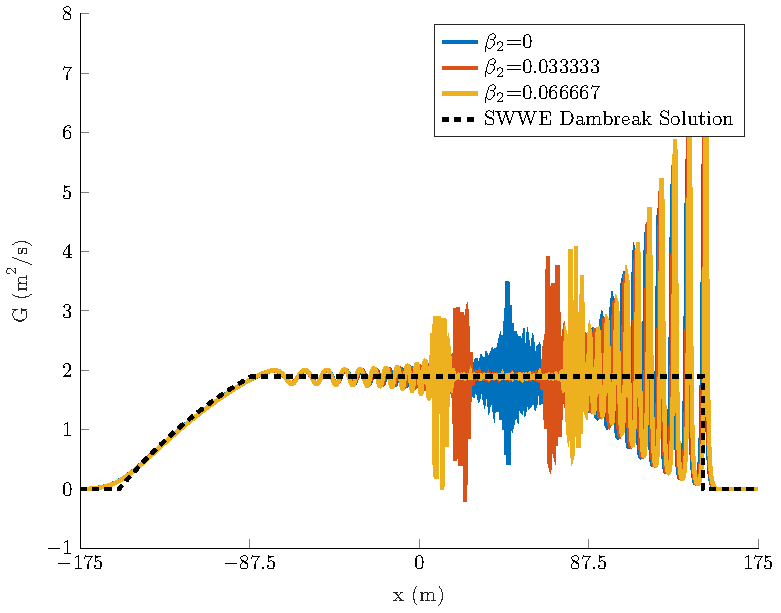
\includegraphics[width=\textwidth]{./Figures/Simulations/Study/ImpDisp/G.pdf}
		\caption{$G$}
	\end{subfigure}
	\begin{subfigure}{0.32\textwidth}
	\centering
	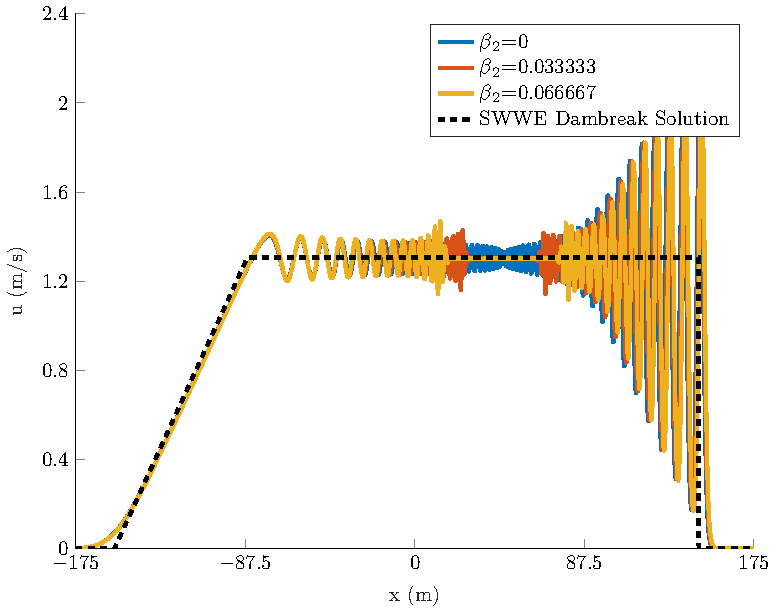
\includegraphics[width=\textwidth]{./Figures/Simulations/Study/ImpDisp/u.pdf}
	\caption{$u$}
	\end{subfigure}
	\caption{Plot of multiple smooth dambreak numerical solutions at $t=35s$.}
\end{figure}

\begin{figure}
	\centering
	\begin{subfigure}{0.32\textwidth}
		\centering
		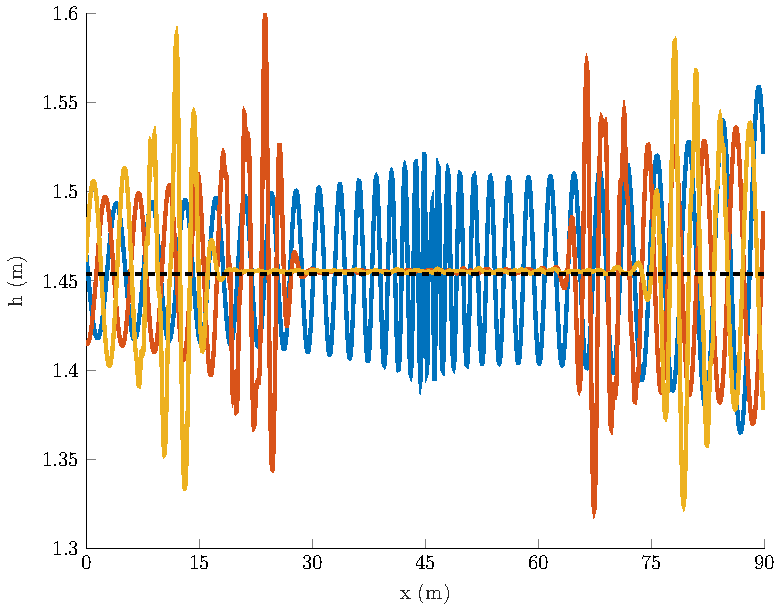
\includegraphics[width=\textwidth]{./Figures/Simulations/Study/ImpDisp/hMiddle.pdf}
		\caption{$h$ in middle of dispersive wave train}
	\end{subfigure}
	\begin{subfigure}{0.32\textwidth}
		\centering
		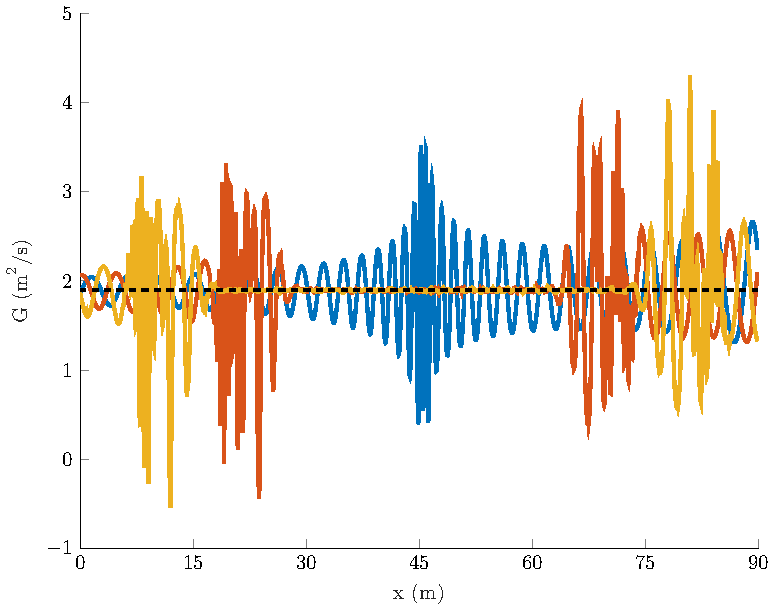
\includegraphics[width=\textwidth]{./Figures/Simulations/Study/ImpDisp/GMiddle.pdf}
		\caption{$G$ in middle of dispersive wave train}
	\end{subfigure}
	\begin{subfigure}{0.32\textwidth}
	\centering
	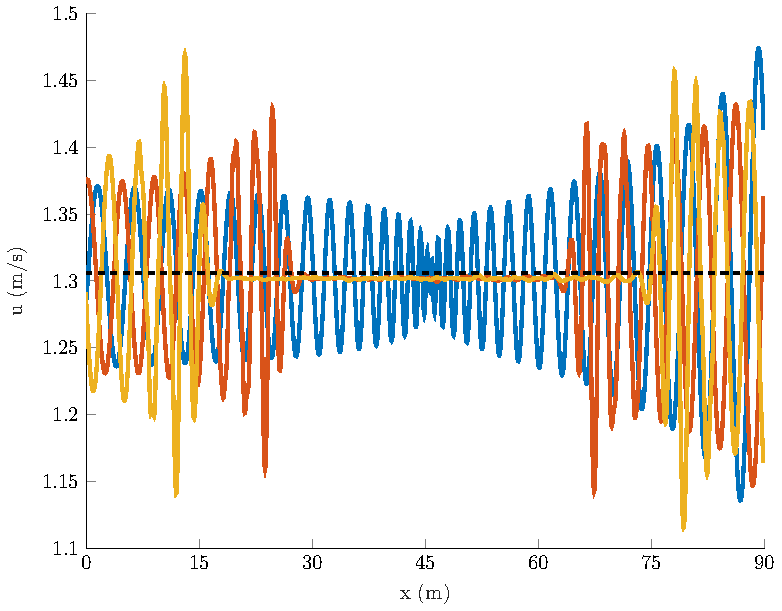
\includegraphics[width=\textwidth]{./Figures/Simulations/Study/ImpDisp/uMiddle.pdf}
	\caption{$u$ in middle of dispersive wave train}
	\end{subfigure}
	\begin{subfigure}{0.32\textwidth}
	\centering
	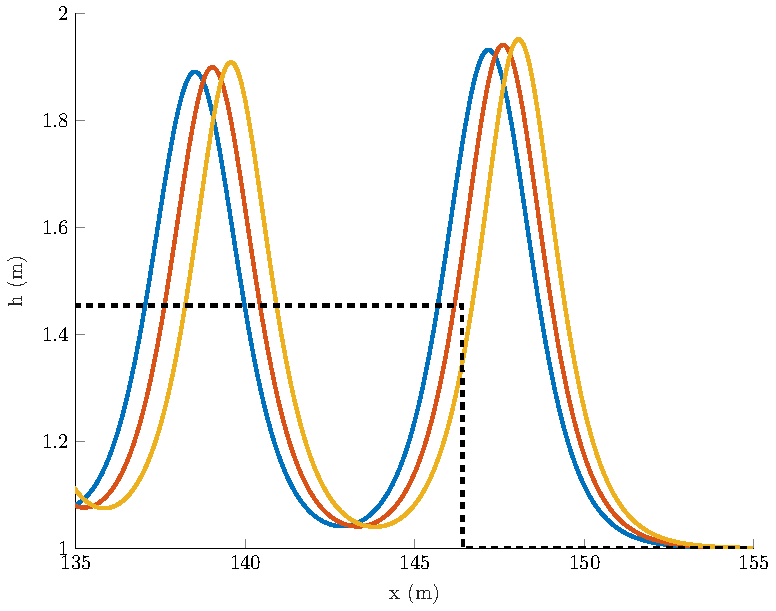
\includegraphics[width=\textwidth]{./Figures/Simulations/Study/ImpDisp/hFront.pdf}
	\caption{$h$ Front of dispersive wave train}
	\end{subfigure}
	\begin{subfigure}{0.32\textwidth}
	\centering
	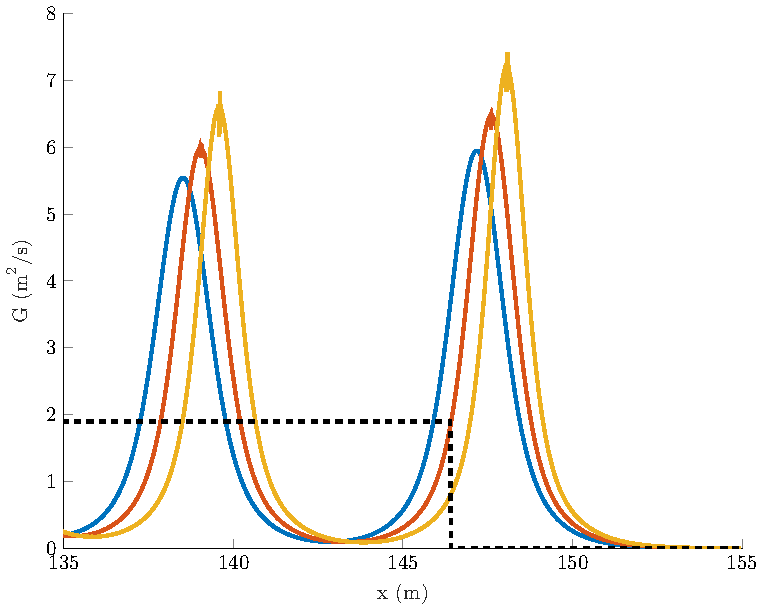
\includegraphics[width=\textwidth]{./Figures/Simulations/Study/ImpDisp/GFront.pdf}
	\caption{$G$ Front of dispersive wave train}
	\end{subfigure}
	\begin{subfigure}{0.32\textwidth}
	\centering
	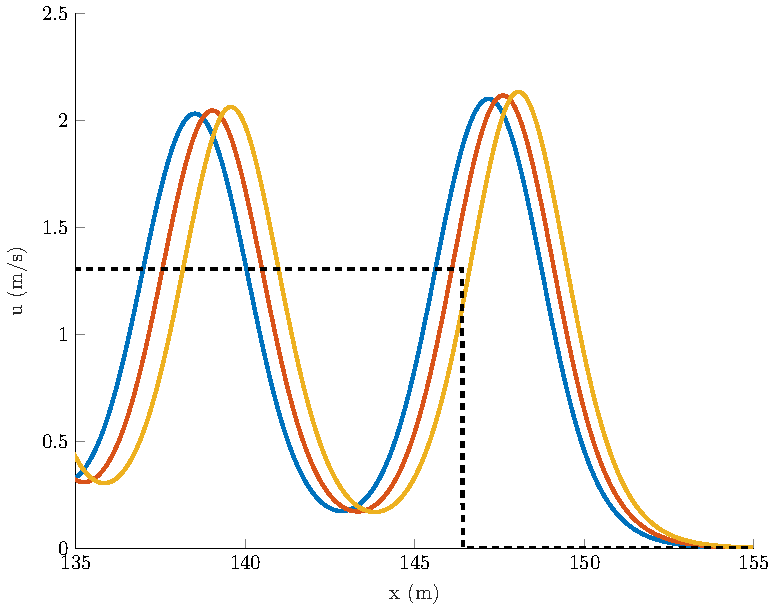
\includegraphics[width=\textwidth]{./Figures/Simulations/Study/ImpDisp/uFront.pdf}
	\caption{$u$ Front of dispersive wave train}
	\end{subfigure}

	\caption{Plot of multiple smooth dambreak numerical solutions at important locations at $t=35s$.}
\end{figure}

\begin{figure}
	\centering
	\begin{subfigure}{0.49\textwidth}
		\centering
		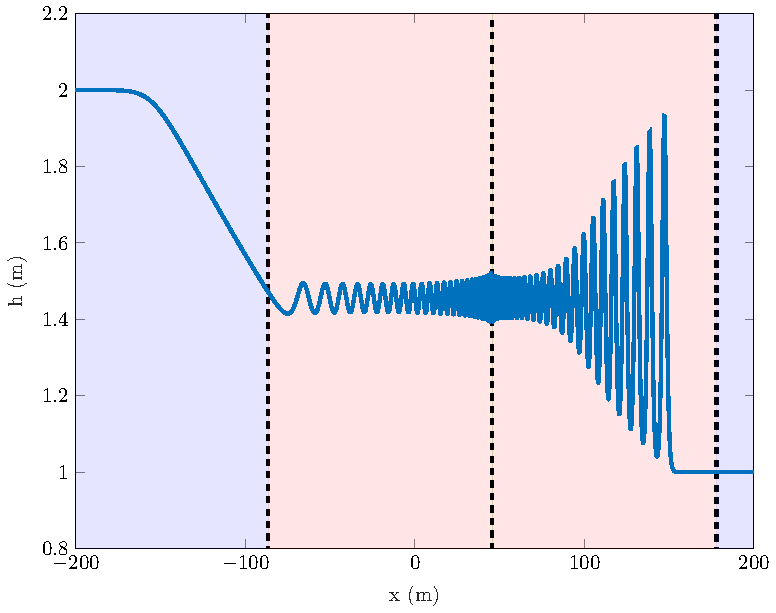
\includegraphics[width=\textwidth]{./Figures/Simulations/Study/ImpDisp/Regions/hRegionsSerre.pdf}
		\caption{$\beta_1 = \beta_2 = 0$}
	\end{subfigure}
	\begin{subfigure}{0.49\textwidth}
		\centering
		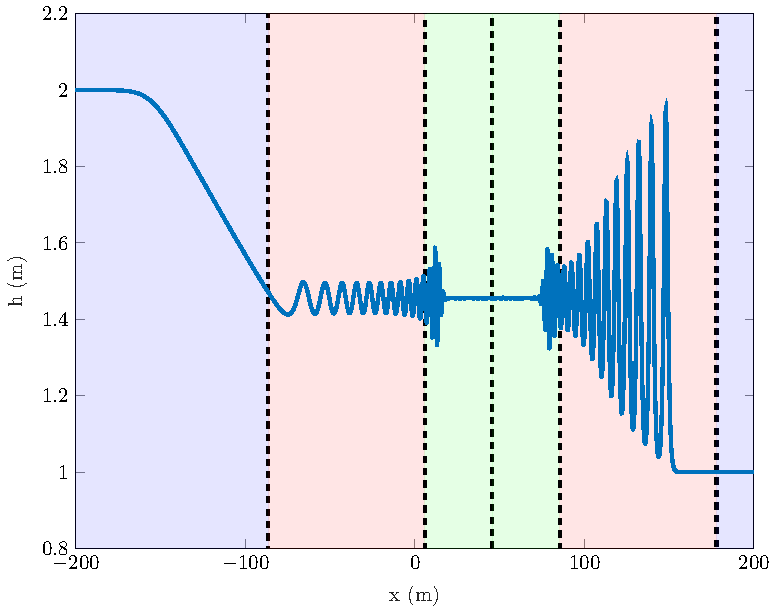
\includegraphics[width=\textwidth]{./Figures/Simulations/Study/ImpDisp/Regions/hRegionsImpDisp.pdf}
		\caption{$\beta_1 = \beta_2 = \frac{1}{15}$}
	\end{subfigure}
	\caption{Regions of wave speeds for the smooth dambreak numerical solution at $t=35s$.}
\end{figure}



\begin{table}
	\centering
	\begin{tabular}{ c | c | c | c | c }
		$\beta_1$ & $h$ & $G$ & $uh$ & $\mathcal{H}$  \\
		\hline
		\T $0$ &	$8.0 \times 10^{-13}$ & $6.3 \times 10^{-13}$  & $3.3 \times 10^{-7}$ &	 $3.8 \times 10^{-6}$ \\
		\T$\dfrac{1}{30}$ & $8.1 \times 10^{-13}$ &	$6.4 \times 10^{-13}$ & $3.5 \times 10^{-7}$	 &	$1.9 \times 10^{-5}$ \\
		\T$\dfrac{1}{15}$ & $8.2 \times 10^{-13}$ &	$6.3 \times 10^{-13}$ & $5.8 \times 10^{-7}$	 &	$1.1 \times 10^{-4}$ \\
		
	\end{tabular}
	\caption{Conservation errors for Modified Dispersion Serre Equations for the solutions provided above with $\beta_2 = \beta_1 $.}
\end{table}



\subsection{Serre To SWWE Family $\beta_2 = 0$ and $-\frac{2}{3} \le \beta_1 \le 0$}
Justify interest, switching dispersion on and off, effect and giving structure/understanding to various schemes that turn it on and off.

Points:
\begin{itemize}
	\item we do get convergence, but most of the convergent behaviour occurs very close to the critical SWWE value. This is because gradients are large in the initial conditions
	\item Middle of dispersive wave train, and base and top of rarefaction fan most affected (closer to Serre)
	\item Still quite a large dispersive wave train even for $\beta_1$ values close to $-2/3$. (This appears to justify switching)
	\item the front of the shock became larger for some intermediate values.
	\item Trade-off between momentum convergence (since G = uh for SWWE) and energy convergence. Dispersive models conserve energy better due to smooth solutions, but conserve momentum worse because conserved quantitiy is not uh. 
\end{itemize}

\begin{figure}
	\centering
	\begin{subfigure}{0.32\textwidth}
		\centering
		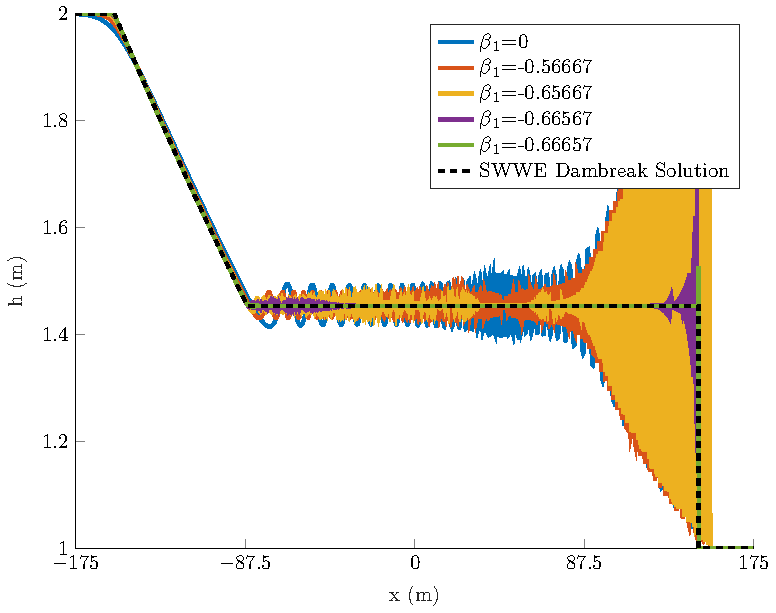
\includegraphics[width=\textwidth]{./Figures/Simulations/Study/Serre2SWWECloser/h.pdf}
		\caption{$h$}
	\end{subfigure}
	\begin{subfigure}{0.32\textwidth}
		\centering
		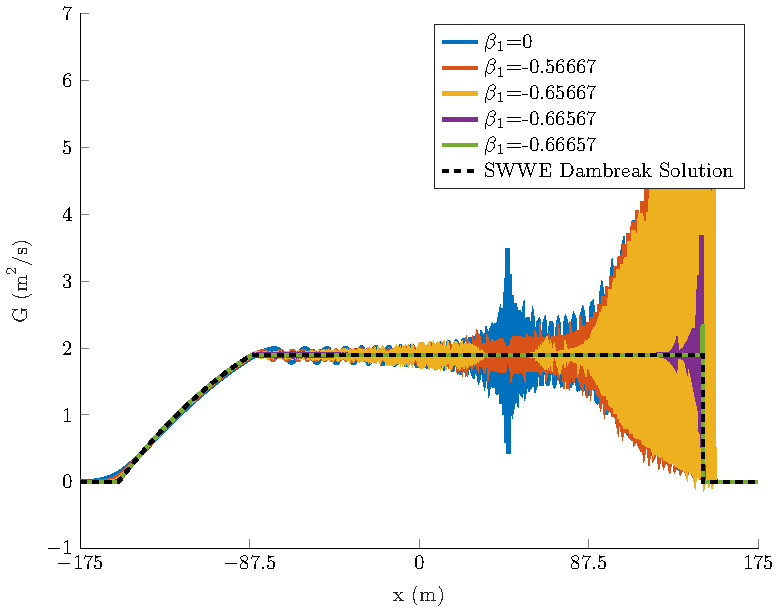
\includegraphics[width=\textwidth]{./Figures/Simulations/Study/Serre2SWWECloser/G.pdf}
		\caption{$G$}
	\end{subfigure}
	\begin{subfigure}{0.32\textwidth}
	\centering
	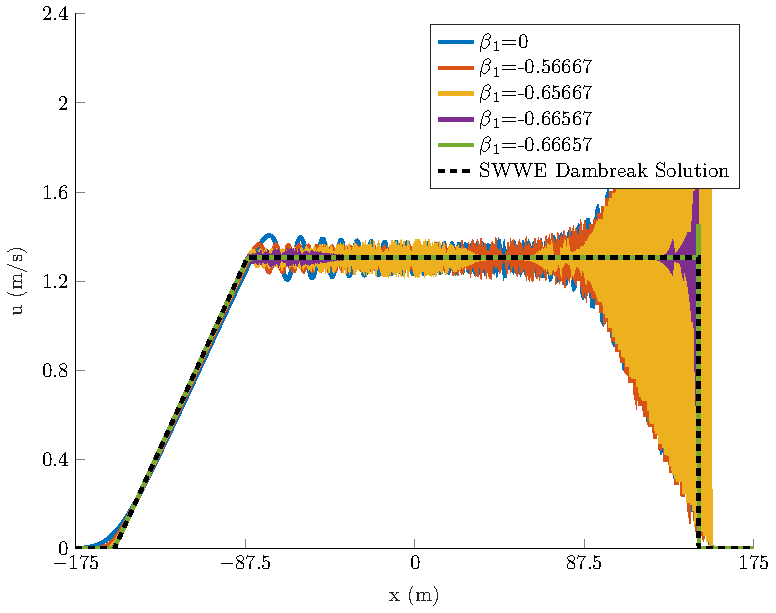
\includegraphics[width=\textwidth]{./Figures/Simulations/Study/Serre2SWWECloser/u.pdf}
	\caption{$u$}
	\end{subfigure}
	\caption{Plot of multiple smooth dambreak numerical solutions at $t=35s$.}
\end{figure}



\begin{figure}
	\centering
	\begin{subfigure}{0.32\textwidth}
		\centering
		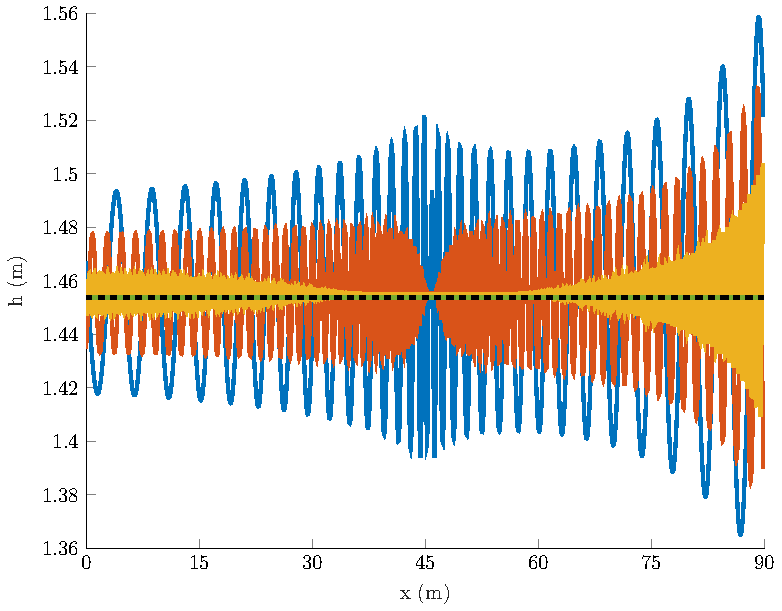
\includegraphics[width=\textwidth]{./Figures/Simulations/Study/Serre2SWWECloser/hMid.pdf}
		\caption{$h$ middle of dispersive wave train}
	\end{subfigure}
	\begin{subfigure}{0.32\textwidth}
		\centering
		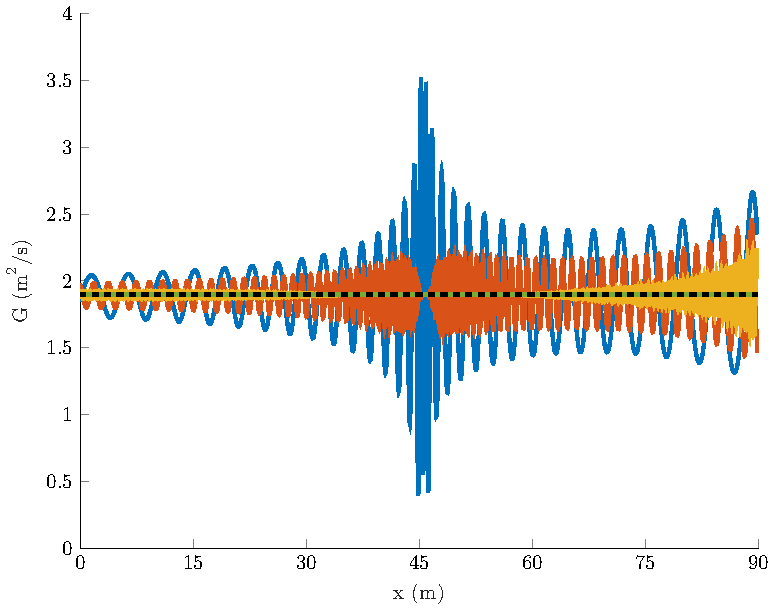
\includegraphics[width=\textwidth]{./Figures/Simulations/Study/Serre2SWWECloser/GMid.pdf}
		\caption{$G$ middle of dispersive wave train}
	\end{subfigure}
	\begin{subfigure}{0.32\textwidth}
		\centering
		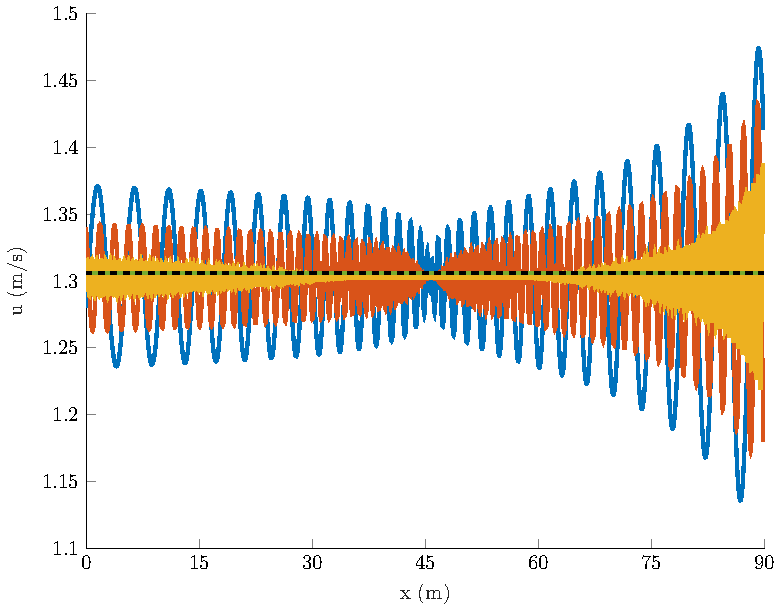
\includegraphics[width=\textwidth]{./Figures/Simulations/Study/Serre2SWWECloser/uMiddle.pdf}
		\caption{$u$ middle of dispersive wave train}
	\end{subfigure}
	\begin{subfigure}{0.32\textwidth}
	\centering
	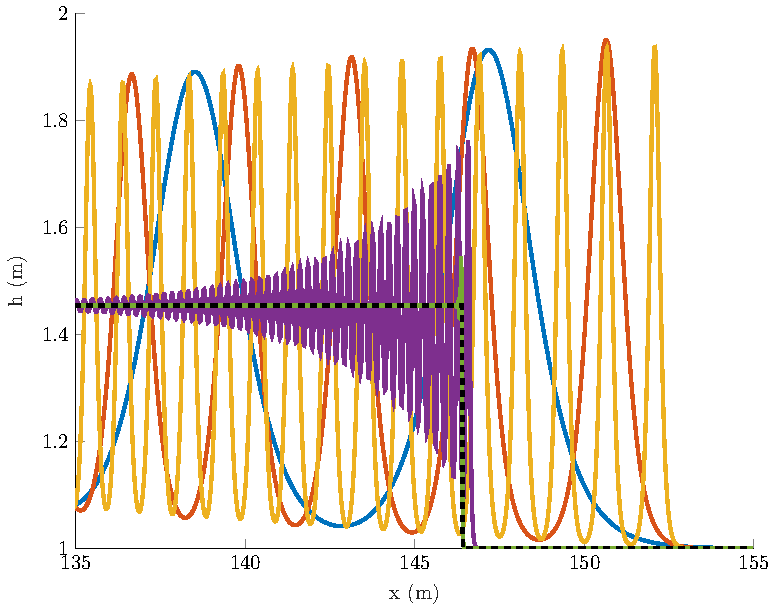
\includegraphics[width=\textwidth]{./Figures/Simulations/Study/Serre2SWWECloser/hFront.pdf}
	\caption{$h$ front of dispersive wave train}
	\end{subfigure}
	\begin{subfigure}{0.32\textwidth}
		\centering
		\includegraphics[width=\textwidth]{./Figures/Simulations/Study/Serre2SWWECloser/GFront.pdf}
		\caption{$G$ front of dispersive wave train}
	\end{subfigure}
	\begin{subfigure}{0.32\textwidth}
		\centering
		\includegraphics[width=\textwidth]{./Figures/Simulations/Study/Serre2SWWECloser/uFront.pdf}
		\caption{$u$ front of dispersive wave train}
	\end{subfigure}
	\caption{Plot of multiple smooth dambreak numerical solutions at $t=35s$.}
\end{figure}


\begin{figure}
	\centering
	\begin{subfigure}{0.49\textwidth}
		\centering
		\includegraphics[width=\textwidth]{./Figures/Simulations/Study/Serre2SWWECloser/Regions/hRegionsSerre.pdf}
		\caption{$\beta_1 = \beta_2 = 0$}
	\end{subfigure}
	\begin{subfigure}{0.49\textwidth}
		\centering
		\includegraphics[width=\textwidth]{./Figures/Simulations/Study/Serre2SWWECloser/Regions/hRegionsSerreSWWEClose.pdf}
		\caption{$\beta_1 = -\frac{2}{3} + 10^{-3}$ and  $\beta_2 = 0$}
	\end{subfigure}
	\caption{Regions of wave speeds for the smooth dambreak numerical solution at $t=35s$.}
\end{figure}


\begin{table}
	\centering
	\begin{tabular}{ c | c | c | c | c }
		$\beta_1$ & $h$ & $G$ & $uh$ & $\mathcal{H}$  \\
		\hline
		\T $0$ &	$8.0 \times 10^{-13}$ &	$6.3 \times 10^{-13}$ & $3.3 \times 10^{-7}$ & $3.8 \times 10^{-6}$ \\
		\T $-\frac{2}{3} + 10^{-1}$ &	$7.2 \times 10^{-13}$ &	$6.3 \times 10^{-13}$ & $3.0 \times 10^{-6}$ & $6.3 \times 10^{-6}$ \\
		\T $-\frac{2}{3} + 10^{-2}$ &	$6.6 \times 10^{-13}$ &	$6.2 \times 10^{-13}$ & $3.2 \times 10^{-5}$ & $3.7 \times 10^{-4}$ \\		
		\T $-\frac{2}{3} + 10^{-3}$ &	$6.0 \times 10^{-13}$ &	$6.3 \times 10^{-13}$ & $1.2 \times 10^{-5}$ & $3.7 \times 10^{-3}$ \\	
		\T $-\frac{2}{3} + 10^{-4}$ &	$5.9 \times 10^{-13}$ &	$6.2 \times 10^{-13}$ & $1.2 \times 10^{-6}$ & $3.7 \times 10^{-3}$ 		
	\end{tabular}
	\caption{Conservation errors for Serre To SWWE Faimly of Equations for the solutions provided above with $\beta_2 = 0$ and $-\frac{2}{3}\le \beta_1 \le 0$.}
\end{table}


\bibliographystyle{unsrtnat}
\bibliography{Bibliography}


\end{document} 